\documentclass[a4paper,11pt,oneside,openany]{iut-thesis}
% برای چاپ پایان‌نامه به صورت دو رو خط فوق را کامنت و خط زیر را فعال کنید همچنین تغییرات لازم برای هدر‌ها را نیز انجام دهید که در ادامه به آن اشاره شده است
%  \documentclass[a4paper,11pt,twoside,openany]{thesis}
\usepackage{amsthm,amssymb,amsmath,textcomp}% فونت‌ها، نمادها و محیط‌های ams
\usepackage{setspace,xargs}
\usepackage{array}%آرایه‌های ریاضی
\usepackage{verbatim}%می‌توان محیط های جدید را با این بسته تعریف نمود
\usepackage{verbatimbox}
\usepackage{indentfirst} %جهت ایجاد تورفتگی در اول پاراگراف
\usepackage{xfrac}
% بسته زیر برای جداول است
\usepackage{tabulary}
\usepackage{colortbl}
\usepackage{framed} 
% بسته زیر برای تنظیمات هدر صفحات است
\usepackage{fancyhdr}
% تنظیم Heading
\usepackage{longtable}
% پکیج برای جداول طولانی
\usepackage{enumitem}
% محیط شمارنده
\usepackage{multicol}
\setlength{\columnsep}{1cm}
% پکیج برای چند ستونی سازی 
%===============================================footnote=====================================
%بسته و تنظیمات زیر زیرنویس هر صفحه را از یک شروع می کند.
\usepackage{zref-perpage}
\zmakeperpage{footnote}
\usepackage{remreset}
\makeatletter
\@removefromreset{footnote}{chapter}
\makeatother
%======================================================================================
\usepackage{tikz,tikz-cd}% برای رسم اشکال و یا نمودارها استفاده می شود. این بسته یکی از مهمترین بسته‌های لاتک است
\usetikzlibrary{shapes.geometric, arrows,patterns}

\usepackage [pagebackref=true, colorlinks, linkcolor=blue, citecolor=magenta, urlcolor=cyan] {hyperref}
% چنانچه قصد پرینت گرفتن نوشته خود را دارید، خط بالا را غیرفعال و  از دستور زیر استفاده کنید. در ضمن pagebackref برای نشان دادن شماره صفحه ارجاعات مراجع در بخش bibliography است.
% \usepackage [pagebackref=false, colorlinks, linkcolor=black, citecolor=black, urlcolor=black] {hyperref}

\usepackage{afterpage}
\usepackage{bookmark}%برای فعال شدن لینک‌ها از این بسته استفاده می شود
% پکیج زیر رنگ و گرافیک و تعریف پوشه عکس‌ها
\usepackage{graphicx,xcolor}

\graphicspath{{./images/}}
\newcommand\figwidth{0.4}
% پکیج زیر برای اضافه کردن کدهای برنامه‌هاست
\usepackage[procnames]{listings}
 \usepackage{lscape}% چنانچه بخواهید صفحه ای را به صورت لندسکیپ درآورید این بسته کمک می کند
\usepackage [a4paper, bindingoffset=-.5cm, footskip=1cm, headheight = 16pt, top=3cm, bottom=2.5cm,  right=3cm,  left=3cm ,] {geometry}% ابعاد صفحه و حاشیه‌ها
% تنظیم ارجاعات
\usepackage[numbers]{natbib}%این بسته برای اضافه نمودن دستورات مرجع زنی مختلف است
% بسته زیر فهرست های  و مراجع را به فهرست مطالب اضافه می کند
\usepackage[nottoc]{tocbibind}
% دو بسته زیر امکان caption را برای عکس‌ها فراهم می نماید
\usepackage[margin=10pt,font=small,labelfont=bf,labelsep=endash]{caption} 
\usepackage[margin=10pt,font=footnotesize,labelfont=bf,labelsep=endash]{subcaption}
\usepackage[xindy,acronym,toc]{glossaries}% اضافه کردن مراجع و نمایه به فهرست مطالب
%بسته زیر امکان ارجاع دهی الکترونیک به مقالات را ایجاد می کند .البته باید استایل مورد استفاده در بخش مراجع دارای تابع doi باشد.استایل های iut-fa و plainnat-faاین آپشن را دارا هستند.
\usepackage{doi}
% خط زیر امکان نوشتن کنار عکس را می دهد
\usepackage{sidecap}
\sidecaptionvpos{figure}{t}
%خط زیر برای خوانش فونت‌ها در ویندوز است.
\usepackage[OT1,EU1]{fontenc}
%خط زیر مراجع را از اولین فصل شماره گذاری می کند و در لیست تصاویر نشان نمی‌دهد.
\usepackage{notoccite}
% در مورد تقدم و تاخر وارد کردن بسته ها تنها باید به چند نکته دقت کرد:
% الف) بسته xepersian حتما حتما باید آخرین بسته ای باشد که فراخوانی می شود
% ب) بسته hyperref جزو آخرین بسته هایی باید باشد که فراخوانی می شود.
% ج) بسته glossaries حتما باید بعد از hyperref فراخوانی شود. 
%  اگر از بسته float استفاده نمی کنید caption جداول مانند تصاویر بسته به اینکه بالا نوشته شده باشند یا پایین تغییر مکان می دهند. چنانچه نیازمندید تا از بسته‌های float که در زیر آمده است استفاده کنید زیرنویس جداول همه در پایین نوشته می شود. برای اینکه زیرنویس‌ها بعد از فعالسازی بسته های float بالا یا پایین جداول نوشته شود حسب انتخاب باید قبل از table مکان را با یکی از دستورات زیر ست نمایید توجه کنید که بعد از دستورات زیر تمامی زیرنویس ها از آن به بعد مطابق با آخرین دستور اعمالی تنظیم می شوند. برای نمونه به جداول فصل چهارم نگاه کنید.
% \usepackage{floatrow}
% \usepackage{morefloats}
% \floatsetup[table]{capposition=bottom}
% \floatsetup[table]{capposition=top}


%%========= Added by Ali =========%%
%\usepackage{subfigure}
%\usepackage{titling}
\newenvironment{rcases}
{\left.\begin{aligned}}
	{\end{aligned}\right\rbrace}

%\usepackage{subfigure}

%%================================%%



%برای نشان دادن رد ماتریس از این عبارت تعریف شده است.می‌توانید عبارات خود را تعریف کنید.
% خط زیر اپراتور تریس را ست می نماید
\DeclareMathOperator{\Tr}{Tr}

%%=========================================== XePersian
%  \usepackage{xepersian}
%اگر می‌خواهید زیرنویس ها تک ستونی شود خط فوق را  فعال کنید و دو خط زیر را غیر فعال کنید

 \usepackage[extrafootnotefeatures]{xepersian}
 \twocolumnfootnotes
\settextfont[Scale=1.1]{Yas}
%\setdigitfont[Scale=1.1]{Yas}
%اگر میخواهید اعداد در فرمولها لاتین باشد خط بالا را کامنت و خط پایین را فعال کنید
\DefaultMathsDigits
\defpersianfont\nastaliq[Scale=2]{IranNastaliq}
\defpersianfont\nastaliqsmal[Scale=1]{IranNastaliq}
\defpersianfont\titr[Scale=1]{XB Titre}
\defpersianfont\traffic[Scale=1]{XM Traffic}
\defpersianfont\nil[Scale=1.3]{XB Niloofar}
% \deflatinfont\urwchl[Scale=1]{Chancery}
% ٫=========================================================
\newcommand\namad[2]{#1\dotfill\lr{#2}\\}
% برای فاصله گذاری استاندارد بین خطوط و دستورات با چند آرگومان اختیاری
%=========================================================================================
% %این خطوط اعداد پانویس‌ها را درست می کند
% \makeatletter
% \footmarkstyle{\textsuperscript{\if@RTL\else\latinfont\fi#1}}
% \makeatother

\makeatletter
\def\@makeLTRfnmark{\hbox{\@textsuperscript{\latinfont\@thefnmark}}}
\renewcommand\@makefntext[1]{%
    \parindent 1em%
    \noindent
    \hb@xt@1.8em{\hss\if@RTL\@makefnmark\else\@makeLTRfnmark\fi}#1}
\makeatother
% %============================================= Counters
% \def\thesection{\arabic{section}-\thechapter}
% \def\thesubsection{\arabic{subsection}-\thesection}
% \def\theequation{\arabic{equation}-\thechapter}
% \def\thetheorem{\arabic{theorem}-\thesection}
% \def\thefigure{\arabic{figure}-\thechapter}
% \def\thetable{\arabic{table}-\thechapter}
% \def\imagetop#1{\vtop{\null\hbox{#1}}}
%\numberwithin{equation}{section}

%
% %خطوط زیر برای تغییر در شکل خط بالای سر پانویسهاست
% \renewcommand{\footnoterule}{%
% 
%   \kern -3pt
%   \hrule width 0.65\textwidth height 0.85pt
%   \kern 2pt
% }
%%%%%%%%%%%%%%%%%%%%%%%%%%%%%%%%%%%%%%%%%%%%%%%%%%%%%%%%%%%%%%%%%%%%%%%%%%%%%%%%%
%

%%%%%%%%%%%%%%%%%%%
\makeatletter
 \def\abj@num@i#1{%
   \ifcase#1\or الف \or ب\or ج\or د%
            \or ه‍\or و\or ز\or ح\or ط\fi
   \ifnum#1=\z@\abjad@zero\fi}   
 \def\@harfi#1{\ifcase#1\or الف\or ب\or پ\or ت\or ث\or
 ج\or چ\or ح\or خ\or د\or ذ\or ر\or ز\or ژ\or س\or ش\or ص\or ض\or ط\or ظ\or ع\or غ\or
 ف\or ق\or ک\or گ\or ل\or م\or ن\or و\or ه\or ی\else\@ctrerr\fi}
 \def\@glsgetgrouptitle#1{\ifcase#1\or الف \or ب\or پ\or ت\or ث\or
 ج\or چ\or ح\or خ\or د\or ذ\or ر\or ز\or ژ\or س\or ش\or ص\or ض\or ط\or ظ\or ع\or غ\or
 ف\or ق\or ک\or گ\or ل\or م\or ن\or و\or ه\or ی\else\@ctrerr\fi}
\makeatother
\makeatletter
\bidi@patchcmd{\@Abjad}{آ}{الف}
{\typeout{Succeeded in changing `آ` into `الف`}}
{\typeout{Failed in changing `آ` into `الف`}}
\makeatother
\PersianAlphs
% خطوط فوق جای آرا با الف عوض می‌کنند.اگر آ را ترجیح می دهید این خطوط را غیرفعال کنید
\makeatletter 
\def\@chapter[#1]#2{\ifnum \c@secnumdepth >\m@ne
                         \refstepcounter{chapter}%
                         \typeout{\@chapapp\space\thechapter.}%
                         \addcontentsline{toc}{chapter}%
                                   {\@chapapp~\protect\numberline{\thechapter}#1}%
                    \else
                      \addcontentsline{toc}{chapter}{#1}%
                    \fi
                    \chaptermark{#1}%
                    \addtocontents{lof}{\protect\addvspace{10\p@}}%
                    \addtocontents{lot}{\protect\addvspace{10\p@}}%
                    \if@twocolumn
                      \@topnewpage[\@makechapterhead{#2}]%
                    \else
                      \@makechapterhead{#2}%
                      \@afterheading
                    \fi}
\renewcommand*\l@section{\@dottedtocline{1}{3.5em}{3.3em}}
\renewcommand*\l@subsection{\@dottedtocline{2}{4.8em}{4.2em}} 
\makeatother
% خطوط فوق تنظیمات فواصل را در فهرست مطالب انجام می دهند اعداد در سه خط پایانی این خطوط مدیر این کارند
% \SepMark{-}
% در فهرست مطالب و ارجاعات اگر می‌خواهید به جای نقطه - بگذارید از خط بالا استفاده کنید.
\makeatletter
\bidi@patchcmd{\Hy@org@chapter}{%
\addcontentsline{toc}{chapter}%
{\protect\numberline{\thechapter}#1}%
}{%
\addcontentsline{toc}{chapter}%
{\protect\numberline{\chaptername~\tartibi{chapter}}#1}%
}{\typeout{We succeded in redefining \string\@chapter}}
{\typeout{We failed in redefining \string\@chapter}}
\bidi@patchcmd{\l@chapter}{%
\setlength\@tempdima{1.5em}%
 }{%
\setlength\@tempdima{3.em}%
}{\typeout{We succeded in redefining \string\l@chapter}}
{\typeout{We failed in redefining \string\l@chapter}}
%تنظیم فاصله پیوست ها در فهرست با خطوط بالاست
%%%%%%%%%%%%%%%%%%%%%%%%%%%%%%%%%%
%%% ============================================================================================================

%%% تنظیمات مربوط به بسته  glossaries
%%% تعریف استایل برای واژه نامه فارسی به انگلیسی، در این استایل واژه‌های فارسی در سمت راست و واژه‌های انگلیسی در سمت چپ خواهند آمد. از حالت گروه ‌بندی استفاده می‌کنیم، 
%%% یعنی واژه‌ها در گروه‌هایی به ترتیب حروف الفبا مرتب می‌شوند، مثلا:
%%% الف
%%% افتصاد ................................... Economy
%%% اشکال ........................................ Failure
%%% ش
%%% شبکه ...................................... Network

\newglossarystyle{myFaToEn}{%
	\renewenvironment{theglossary}{}{}
	\renewcommand*{\glsgroupskip}{\vskip 10mm}
	\renewcommand*{\glsgroupheading}[1]{\subsection*{\glsgetgrouptitle{##1}}}
	\renewcommand*{\glossentry}[2]{\begin{flushleft}\noindent\glsentryname{##1}{،##2}\dotfill\space\glsentrytext{##1}\end{flushleft}
	}
}

%% % تعریف استایل برای واژه نامه انگلیسی به فارسی، در این استایل واژه‌های فارسی در سمت راست و واژه‌های انگلیسی در سمت چپ خواهند آمد. از حالت گروه ‌بندی استفاده می‌کنیم، 
%% % یعنی واژه‌ها در گروه‌هایی به ترتیب حروف الفبا مرتب می‌شوند، مثلا:
%% % E
%%% Economy ............................... اقتصاد
%% % F
%% % Failure................................... اشکال
%% %N
%% % Network ................................. شبکه

\newglossarystyle{myEntoFa}{%
	%%% این دستور در حقیقت عملیات گروه‌بندی را انجام می‌دهد. بدین صورت که واژه‌ها در بخش‌های جداگانه گروه‌بندی می‌شوند، 
	%%% عنوان بخش همان نام حرفی است که هر واژه در آن گروه با آن شروع شده است. 
	\renewenvironment{theglossary}{}{}
	\renewcommand*{\glsgroupskip}{\vskip 10mm}
	\renewcommand*{\glsgroupheading}[1]{\begin{LTR} \subsection*{\glsgetgrouptitle{##1}} \end{LTR}}
	%%% در این دستور نحوه نمایش واژه‌ها می‌آید. در این جا واژه فارسی در سمت راست و واژه انگلیسی در سمت چپ قرار داده شده است، و بین آن با نقطه پر می‌شود. 
	\renewcommand*{\glossentry}[2]{\begin{flushleft}\glsentrytext{##1}\noindent\dotfill\space \lr{\glsentryname{##1}{ ,##2}}\end{flushleft}	
	}
}

%%% تعیین استایل برای فهرست اختصارات
\newglossarystyle{myAbbrlist}{%
	%%% این دستور در حقیقت عملیات گروه‌بندی را انجام می‌دهد. بدین صورت که اختصارات‌ در بخش‌های جداگانه گروه‌بندی می‌شوند، 
	%%% عنوان بخش همان نام حرفی است که هر اختصار در آن گروه با آن شروع شده است. 
	\renewenvironment{theglossary}{}{}
	\renewcommand*{\glsgroupskip}{\vskip 10mm}
	\renewcommand*{\glsgroupheading}[1]{\begin{LTR} \subsection*{\glsgetgrouptitle{##1}} \end{LTR}}
	%%% در این دستور نحوه نمایش اختصارات می‌آید. در این جا حالت کوچک اختصار در سمت چپ و حالت بزرگ در سمت راست قرار داده شده است، و بین آن با نقطه پر می‌شود. 
	\renewcommand*{\glossentry}[2]{\noindent\glsentrytext{##1}\lr{##2,}\dotfill\space \Glsentrylong{##1}
		
	}
	%%% تغییر نام محیط abbreviation به فهرست اختصارات
	\renewcommand*{\acronymname}{\rl{فهرست اختصارات}}
}

%%% برای اجرا xindy بر روی فایل .tex و تولید واژه‌نامه‌ها و فهرست اختصارات و فهرست نمادها یکسری  فایل تعریف شده است.‌ Latex داده های مربوط به واژه نامه و .. را در این 
%%%  فایل‌ها نگهداری می‌کند. مهم‌ترین option‌ این قسمت این است که 
%%% عنوان واژه‌نامه‌ها و یا فهرست اختصارات و یا فهرست نمادها را می‌توانید در این‌جا مشخص کنید. 
%%% در این جا عباراتی مثل glg، gls، glo و ... پسوند فایل‌هایی است که برای xindy بکار می‌روند. 
\newglossary[glg]{english}{gls}{glo}{واژه‌نامه انگلیسی به فارسی}
\newglossary[blg]{persian}{bls}{blo}{واژه‌نامه فارسی به انگلیسی}
\makeglossaries
\glsdisablehyper
%%% تعاریف مربوط به تولید واژه نامه و فهرست اختصارات و فهرست نمادها
%%%  در این فایل یکسری دستورات عمومی برای وارد کردن واژه‌نامه آمده است.
%%%  به دلیل این‌که قرار است این دستورات پایه‌ای را بازنویسی کنیم در این‌جا تعریف می‌کنیم. 
\let\oldgls\gls
\let\oldglspl\glspl

\makeatletter

\renewrobustcmd*{\gls}{\@ifstar\@msgls\@mgls}
\newcommand*{\@mgls}[1] {\ifthenelse{\equal{\glsentrytype{#1}}{english}}{\oldgls{#1}\glsuseri{f-#1}}{\lr{\oldgls{#1}}}}
\newcommand*{\@msgls}[1]{\ifthenelse{\equal{\glsentrytype{#1}}{english}}{\glstext{#1}\glsuseri{f-#1}}{\lr{\glsentryname{#1}}}}

\renewrobustcmd*{\glspl}{\@ifstar\@msglspl\@mglspl}
\newcommand*{\@mglspl}[1] {\ifthenelse{\equal{\glsentrytype{#1}}{english}}{\oldglspl{#1}\glsuseri{f-#1}}{\oldglspl{#1}}}
\newcommand*{\@msglspl}[1]{\ifthenelse{\equal{\glsentrytype{#1}}{english}}{\glsplural{#1}\glsuseri{f-#1}}{\glsentryplural{#1}}}

\makeatother

\newcommand{\newword}[4]{
	\newglossaryentry{#1}     {type={english},name={\lr{#2}},plural={#4},text={#3},description={}}
	\newglossaryentry{f-#1} {type={persian},name={#3},text={\lr{#2}},description={}}
}

%%% بر طبق این دستور، در اولین باری که واژه مورد نظر از واژه‌نامه وارد شود، پاورقی زده می‌شود. 
\defglsentryfmt[english]{\glsgenentryfmt\ifglsused{\glslabel}{}{\LTRfootnote{\glsentryname{\glslabel}}}}

%%% بر طبق این دستور، در اولین باری که واژه مورد نظر از فهرست اختصارات وارد شود، پاورقی زده می‌شود. 
\defglsentryfmt[acronym]{\glsentryname{\glslabel}\ifglsused{\glslabel}{}{\LTRfootnote{\glsentrydesc{\glslabel}}}}


%%%%%% ================================================ دستور برای قرار دادن فهرست اختصارات 
\newcommand{\printabbreviation}{
	\cleardoublepage
	\phantomsection
	\baselineskip=.75cm
	%% با این دستور عنوان فهرست اختصارات به فهرست مطالب اضافه می‌شود. 
%	\addcontentsline{toc}{chapter}{فهرست اختصارات}
	\setglossarystyle{myAbbrlist}
	\begin{LTR}
		\Oldprintglossary[type=acronym]	
	\end{LTR}
	\clearpage
}%

\newcommand{\printacronyms}{\printabbreviation}
%%% در این جا محیط هر دو واژه نامه را باز تعریف کرده ایم، تا اولا مشکل قرار دادن صفحه اضافی را حل کنیم، ثانیا عنوان واژه نامه ها را با دستور addcontentlist وارد فهرست مطالب کرده ایم.
\let\Oldprintglossary\printglossary
\renewcommand{\printglossary}{
	\let\appendix\relax
	%% تنظیم کننده فاصله بین خطوط در این قسمت
	\clearpage
	\phantomsection
	%% این دستور موجب این می‌شود که واژه‌نامه‌ها در  حالت دو ستونی نوشته شود. 
	\twocolumn{}
	%% با این دستور عنوان واژه‌نامه به فهرست مطالب اضافه می‌شود. 
% 	\addcontentsline{toc}{chapter}{واژه نامه انگلیسی به فارسی}
	\setglossarystyle{myEntoFa}
	\Oldprintglossary[type=english]
	
	\clearpage
	\phantomsection
	%% با این دستور عنوان واژه‌نامه به فهرست مطالب اضافه می‌شود. 
% 	\addcontentsline{toc}{chapter}{واژه نامه فارسی به انگلیسی}
	\setglossarystyle{myFaToEn}
	\Oldprintglossary[type=persian]
	\onecolumn{}
}%
%%%%%% ============================================================================================================
%%%%%% 

%
%%============================================ Titles
\renewcommand{\abstractname}{\Large چکیده}
\renewcommand{\listfigurename}{فهرست تصاویر}
%\renewcommand{\latinabstract}{}
\renewcommand{\proofname}{\textbf{برهان}}
\renewcommand{\qedsymbol}{$\blacksquare$}
\renewcommand{\bibname}{مراجع}

% \newcommand*{\doi}[1]{doi:\href*{http://dx.doi.org/#1}{#1}}
% for figures: caption label is italic, the caption text is bold / italic
%\captionsetup[figure]{labelfont={bf,it},textfont={normalfont,it}}
% for subfigures: caption label is bold, the caption text normal.
% justification is raggedright (i.e. left aligned)
% singlelinecheck=off means that the justification setting is used even when the caption is only a single line long. 
% if singlelinecheck=on, then caption is always centered when the caption is only one line.
%\captionsetup[subfigure]{labelfont=normalfont,textfont=bf,singlelinecheck=off,justification=raggedright}
%\captionsetup{textfont=rm,justification=centering,labelsep=newline}
%%======================================== Environments
\newcounter{theorem}[section]
\newcommand{\environ}[2]{\vspace{7pt} \refstepcounter{theorem}\par\noindent  \textbf{\hboxR{#1}\space\thetheorem} \textbf{\space\hboxR{#2}} \\[5pt]}
\newcommand{\closeenviron}{\par\vspace{3pt}}
\newenvironment{thm}[1][]{\environ{قضیه}{#1}\it}{\closeenviron}
\newenvironment{lem}[1][]{\environ{لم}{#1}\it}{\closeenviron}
\newenvironment{prop}[1][]{\environ{گزاره}{#1}\it}{\closeenviron}
\newenvironment{cor}[1][]{\environ{نتیجه}{#1}\it}{\closeenviron}
\newenvironment{con}[1][]{\environ{حدس}{#1}\it}{\closeenviron}
\newenvironment{dfn}[1][]{\environ{تعریف}{#1}\rm}{‌\hfill $\blacktriangle$ \closeenviron}
\newenvironment{notation}[1][]{\environ{نماد}{#1}\rm}{‌\hfill $\blacktriangledown$ \closeenviron}
\newenvironment{rem}[1][]{\environ{ملاحظه}{#1}\rm}{‌\hfill $\blacklozenge$ \closeenviron}
\newenvironment{exm}[1][]{\environ{مثال}{#1}\rm}{‌\hfill $\bigstar$ \closeenviron}
%
\makeatletter
\newenvironment{prob}[4][]{\@ifempty{#1}
{\vspace{15pt} \par\noindent
\parbox{15cm}{\hskip 7pt\underline{\bf #2}\\[4pt]
\begin{tabular}{p{40pt}l}
\textbf{نمونه:}& \parbox[t]{11.8cm}{#3}\\[7pt]
\textbf{سوال:}& \parbox[t]{11.8cm}{#4}
\end{tabular}\vspace{5pt}
}}
{\vspace{5pt} \par\noindent
\parbox{15cm}{\hskip 7pt\underline{\bf #2}\\[4pt]
\begin{tabular}{p{40pt}l}
\textbf{ثابت‌ها:}& \parbox[t]{11.5cm}{#1}\\[4pt]
\textbf{نمونه:}& \parbox[t]{11.5cm}{#3}\\[7pt]
\textbf{سوال:}& \parbox[t]{11.5cm}{#4}
\end{tabular}\vspace{5pt}
}}} {\\[5pt]}
\makeatother

%

%%======================================== Main body
%


\headheight = 20pt
\pagestyle{plain}
\fancyhf{}
% \lhead{\thepage}
% \rhead{\leftmark}
\doublespacing
\allowdisplaybreaks[1]
% اجازه برای شکستن صفحه در وسط محیط ریاضی
%\setlength{\parindent}{1cm} %دستور برای مشخص کردن فاصله ابتدای هر پاراگراف

% %%%%% ============================================================================================================
% % فرامین مربوط به تعیین رنگ و استفاده از آنها در قسمت کد های برنامه نویسی
\definecolor{keywords}{RGB}{255,0,90}
\definecolor{comments}{RGB}{0,0,205}
\definecolor{red}{RGB}{160,0,0}
\definecolor{green}{RGB}{0,150,0}
 \definecolor{Background}{rgb}{0.98,0.98,0.98}
 \definecolor{Keywords}{rgb}{0,0,1}
  \definecolor{Black}{RGB}{0,0,0}
 \definecolor{VioletRed}{RGB}{208,32,144}
 \definecolor{DarkOliveGreen}{RGB}{85,107,47}
 \definecolor{Saddle Brown}{RGB}{139,69,19}
 \definecolor{juliacomment}{RGB}{204,204,0}
 
%  تنظیمات زیر برای رنگ بندی کد بش است
  \lstdefinestyle{Mybash}{ language = Bash,
  literate = {\$\#}{{{\$\#}}}2,
  columns  = fullflexible,
 basicstyle=\ttfamily\scriptsize, 
        keywordstyle=\color{DarkOliveGreen}\bfseries,
        commentstyle=\color{comments}\bfseries,
        stringstyle=\color{green}\bfseries,
        showstringspaces=false,
        identifierstyle=\color{Black}\bfseries,
        procnamekeys={cp,sudo,chmod,fplo2wannier},
        prebreak=\raisebox{0ex}[0ex][0ex]{\ensuremath{\hookleftarrow}},
        numbers=left,
        numberstyle=\footnotesize\color{Saddle Brown},
        breaklines=true,  
        numbersep=5pt,
        captionpos=b,   
        backgroundcolor=\color{Background}\bfseries,
        tabsize=2,
        morekeywords={[2]},
        keywordstyle={[2]\color{VioletRed}\bfseries},
        morekeywords={[3],kmeshfplo,cp,bash,sudo,chmod,fplo2wannier,apt-get},
        keywordstyle={[3]\color{DarkOliveGreen}\bfseries},
        emph={self},
        emphstyle={\color{self}\bfseries},
        frame=1
	}
 \lstdefinestyle{Tex}{ language = Tex,
  literate = {\$\#}{{{\$\#}}}2,
  columns  = fullflexible,
    escapeinside={\%*}{*)},
      morekeywords={encoding,
        xs:schema,xs:element,xs:complexType,xs:sequence,xs:attribute},
 basicstyle=\ttfamily\scriptsize, 
        keywordstyle=\color{DarkOliveGreen}\bfseries,
        commentstyle=\color{comments}\bfseries,
        stringstyle=\color{green}\bfseries,
        showstringspaces=false,
        identifierstyle=\color{Black}\bfseries,
         procnamekeys={end,begin,documentclass,usepackage},
        prebreak=\raisebox{0ex}[0ex][0ex]{\ensuremath{\hookleftarrow}},
        numbers=left,
        numberstyle=\footnotesize\color{Saddle Brown},
        breaklines=true,  
        numbersep=5pt,
        captionpos=b,   
        backgroundcolor=\color{Background}\bfseries,
        tabsize=2,
        morekeywords={[2]amsmath,amssymb,amsthm,array,babel,biblatex,bm,booktabs,boxedminipage,caption,cancel,chemmacros,changepage,cleveref,dcolumn,enumitem,epstopdf,esint,eucal,fancyhdr,float,fontenc,gensymb,geometry,glossaries,graphicx,grffile,hyperref,indentfirst,inputenc,latexsym,listings,longtable,mathptmx,mathrsfs,mathtools,mhchem,microtype,multicol,natbib,pdfpages,rotating,setspace,showkeys,showidx,subfiles,subcaption,syntonly,textcomp,theorem,todonotes,siunitx,ulem,url,verbatim,xcolor,xypic},
        keywordstyle={[2]\color{VioletRed}\bfseries},
%         morekeywords={[3]},
%         keywordstyle={[3]end,begin,documentclass,usepackage \color{DarkOliveGreen}\bfseries},
        emph={self},
        emphstyle={\color{self}\bfseries},
        frame=1
	}
% تنظیمات زیر برای رنگبندی کد Python‌است
 \lstdefinestyle{Mypython}{language=Python, 
 basicstyle=\ttfamily\scriptsize, 
        sensitive=true,
        keywordstyle=\color{Keywords}\bfseries,
        commentstyle=\color{comments}\bfseries,
        stringstyle=\color{green}\bfseries,
        showstringspaces=false,
        identifierstyle=\color{Black}\bfseries,
        procnamekeys={def,class},
        prebreak=\raisebox{0ex}[0ex][0ex]{\ensuremath{\hookleftarrow}},
        numbers=left,
        numberstyle=\footnotesize\color{Saddle Brown},
        breaklines=true,  
        numbersep=5pt,
        captionpos=b,   
        backgroundcolor=\color{Background}\bfseries,
        tabsize=2,
        morekeywords={[2]@invariant},
        keywordstyle={[2]\color{VioletRed}\bfseries},
        morekeywords={[3],reshape,sin,cos,exp,conjugate,shape,pi,sqrt,genfromtxt,isclose,arctan,complex,dot,arccos,array,float64,sum,multiply,divide,subtract,add,nan_to_num,arctan2,zeros},
        keywordstyle={[3]\color{DarkOliveGreen}\bfseries},
        emph={self},
        emphstyle={\color{self}\bfseries},
        frame=1
	}
% تنظیمات برای رنگ بندی کد C است
\definecolor{mGreen}{rgb}{0,0.6,0}
\definecolor{mGray}{rgb}{0.5,0.5,0.5}
\definecolor{mPurple}{rgb}{0.58,0,0.82}
\definecolor{backgroundColour}{rgb}{0.95,0.95,0.92}
\definecolor{mygreen}{RGB}{28,172,0} % color values Red, Green, Blue
\definecolor{mylilas}{RGB}{170,55,241}
\lstdefinestyle{CStyle}{
    backgroundcolor=\color{backgroundColour},   
    commentstyle=\color{mGreen},
    keywordstyle=\color{magenta},
    numberstyle=\scriptsize\color{Saddle Brown},
    stringstyle=\color{mPurple},
 basicstyle=\ttfamily\scriptsize, 
    breakatwhitespace=false,         
    breaklines=true,                 
    captionpos=b,                    
    keepspaces=true,                 
    numbers=left,                    
    numbersep=5pt,                  
    showspaces=false,                
    showstringspaces=false,
    showtabs=false,                  
    tabsize=2,
    language=C
}
\lstdefinestyle{julia}
{
  keywordsprefix=\@,
  morekeywords={,exit,whos,edit,load,is,isa,isequal,typeof,tuple,ntuple,uid,hash,finalizer,convert,promote,
    subtype,typemin,typemax,realmin,realmax,sizeof,eps,promote_type,method_exists,applicable,
    invoke,dlopen,dlsym,system,error,throw,assert,new,Inf,Nan,pi,im,begin,while,for,in,return,
    break,continue,macro,quote,let,for,function,println,while,
    if,elseif,else,try,catch,end,bitstype,ccall,do,using,module,
    import,export,importall,baremodule,immutable,local,global,const,Bool
  },
  sensitive=true,
  alsoother={$},%
   morecomment=[l]\#,%
   morecomment=[n]{\#=}{=\#},%
   morestring=[s]{"}{"},%
   morestring=[m]{'}{'},%
basicstyle=\ttfamily\scriptsize, 
        sensitive=true,
        keywordstyle=\color{Keywords}\bfseries,
        commentstyle=\color{juliacomment}\bfseries,
        stringstyle=\color{green}\bfseries,
        showstringspaces=false,
        identifierstyle=\color{Black}\bfseries,
        procnamekeys={def,class},
        prebreak=\raisebox{0ex}[0ex][0ex]{\ensuremath{\hookleftarrow}},
        numbers=left,
        numberstyle=\footnotesize\color{Saddle Brown},
        breaklines=true,  
        numbersep=5pt,
        captionpos=b,   
        backgroundcolor=\color{backgroundColour}\bfseries,
         morekeywords={[3],reshape,sin,cos,exp,conjugate,shape,pi,sqrt,genfromtxt,isclose,arctan,complex,dot,arccos,array,float64,sum,multiply,divide,subtract,add,nan_to_num,arctan2,zeros,Int,Int8,Int16,Int32,rand,randn,trace,lolog,diag,eye,linespace,grid
    Int64,Uint,Uint8,Uint16,Uint32,Uint64,Float32,Float64,Complex64,Complex128,Any,Nothing,None,type,typealias,abstract},
           keywordstyle={[3]\color{DarkOliveGreen}\bfseries},
        tabsize=2,
        emph={self},
        emphstyle={\color{self}\bfseries},
        frame=1
}
\definecolor{mygreen}{rgb}{0,0.6,0}
\definecolor{mygray}{rgb}{0.5,0.5,0.5}
\definecolor{mymauve}{rgb}{0.58,0,0.82}
\lstdefinestyle{mymatlab}{language=Matlab,%
  basicstyle=\ttfamily\scriptsize,         % size of fonts used for the code
    %basicstyle=\color{red},
    backgroundcolor=\color{backgroundColour},   
    breaklines=true,%
    morekeywords={matlab2tikz},
      captionpos=b,                    % sets the caption-position to bottom
    keywordstyle=\color{blue},%
%     morekeywords=[2]{1}, keywordstyle=[2]{\color{black}},
    identifierstyle=\color{black},%
    stringstyle=\color{mylilas},
    commentstyle=\color{mygreen},%
    showstringspaces=false,%without this there will be a symbol in the places where there is a space
    numbers=left,%
    numberstyle={\tiny \color{black}},% size of the numbers
    numbersep=9pt, % this defines how far the numbers are from the text
    emph=[1]{for,end,break},emphstyle=[1]\color{red}, %some words to emphasise
    numberstyle=\footnotesize\color{Saddle Brown}
    %emph=[2]{word1,word2}, emphstyle=[2]{style},    
}
\lstdefinestyle{myfortran}{language=[90]Fortran,
backgroundcolor=\color{backgroundColour},   
  morecomment=[l]{!\ }% Comment only with space after !
   backgroundcolor=\color{white},   % choose the background color
 basicstyle=\ttfamily\scriptsize,         % size of fonts used for the code
  breaklines=true,                 % automatic line breaking only at whitespace
  captionpos=b,                    % sets the caption-position to bottom
  commentstyle=\color{mygreen},    % comment style
  escapeinside={\%*}{*)},          % if you want to add LaTeX within your code
  keywordstyle=\color{blue},       % keyword style
  stringstyle=\color{mymauve},     % string literal style
  numbers=left,
  numberstyle=\footnotesize\color{Saddle Brown},
}
%=====================================================

\XeTeXinterchartokenstate=1
%دستوری برای اینکه کشیدگی در کلمات ایجاد شود
\abovedisplayshortskip=10pt
\belowdisplayshortskip=8pt
%دستوری برای تنظیم فاصله عمودی قبل و بعد از فرمول‌ها


\begin{document}
	
%%===============================TITLE===============================%%

\university{
	دانشگاه صنعتی اصفهان
}
\department{
	دانشکده فیزیک
}
\type{
	گزارش پروژه
}
\degree{
	درس
}
\subject{
	مکانیک کوانتومی ۲
}
\field{
}
\title{
	نظریه نوسانات نوترینو و معرفی آزمایش KATRIN برای محاسبه جرم نوترینو
}
\tit{}
\supervisor{
	دکتر مهدی عبدی
}
\secsupervisor{
}
\advisor{
}
\secadvisor{} 
\author{
	علی صالحی
}
\thesisdate{\today}

\makefatitle

%%===============================TITLE===============================%%

%%===============================ABSTRACT===============================%%

\begin{abstract}
در این گزارش ابتدا با نوترینوها و تاریخچه حضورشان در فیزیک آشنا می‌شویم. سپس نظریه نوسانات نوترینو، که جرم دار بودن آنها را ایجاب می‌کند را شرح داده و محاسبه‌ای برای به دست آوردن جرم نوترینو در حالت ایده‌آل انجام می‌دهیم. در آخر با معرفی یکی از مهمترین آزمایشگاه‌های نوترینویی حال حاضر دنیا، برخی چالش‌های آزمایشگاهی برای محاسبه جرم این ذره مرموز را بررسی می‌کنیم. آزمایش KATRIN قرار است با روشی مستقل از مدل، جرم نوترینو را تعیین و یا حد جرمی جدیدی برای آن پیدا کند.
\end{abstract}
\newpage

\tableofcontents

\newpage
%%===============================ABSTRACT===============================%%

%%===============================SECTION-1===============================%%

\section{
مقدمه (تاریخچه کشف نوترینو)
}
در دهه ۱۹۳۰ میلادی مشکلی در مطالعات واپاشی بتازا به وجود آمده بود. در واپاشی بتازا، یک هسته مادر (A) با انتشار یک الکترون به یک هسته دختر با جرم کمی کمتر (B) تبدیل می‌شود:
\begin{equation}
A \rightarrow B + e^{-}\,.
\end{equation}
قانون پایستگی بار حکم می‌کند که بار هسته دختر یک واحد بیشتر از هسته مادر باشد. امروزه می‌دانیم در این واپاشی در واقع یک نوترون به یک پروتون تبدیل شده است. از واپاشی‌های بتازای معروف می‌توان به تبدیل پتاسیم به کلسیم
$({^{40}_{19}K} \rightarrow {^{40}_{20}Ca})$
، مس به روی
$({^{64}_{29}Cu} \rightarrow {^{64}_{30}Zn})$
و تریتیوم به هلیوم
$({^{3}_{1}H} \rightarrow {^{3}_{2}He})$
 اشاره کرد.

در دو جسم (همانند واپاشی آلفازا) می‌توان انرژی‌های ذرات تولید شده را دقیقا محاسبه کرد. در دستگاه مرکز جسم هسته مادر، هسته دختر و الکترون گسیل شده باید در جهات مخالف هم و با تکانه‌های هم اندازه وابپاشند. پس طبق اصل پایستگی انرژی انرژی الکترون از رابطه زیر محاسبه می‌شود:
\begin{equation}\label{Emax}
E = (\frac{{m_{A}}^2 - {m_{B}}^2 + {m_{e}}^2}{2 m_{A}})\,.
\end{equation}
این معادله به ما می‌گوید هنگامی که سه جرم بالا معین باشند، انرژی الکترون باید مقداری ثابت داشته باشد.  اما در آزمایشگاه دیده شد که الکترون‌های گسیل شده طیف وسیعی از انرژی‌ها را دارا هستند و معادله 
(\ref{Emax}) 
فقط بیشینه انرژی الکترون را تعیین می‌کند. 
(
شکل 
\ref{betaspec})

\begin{figure}
	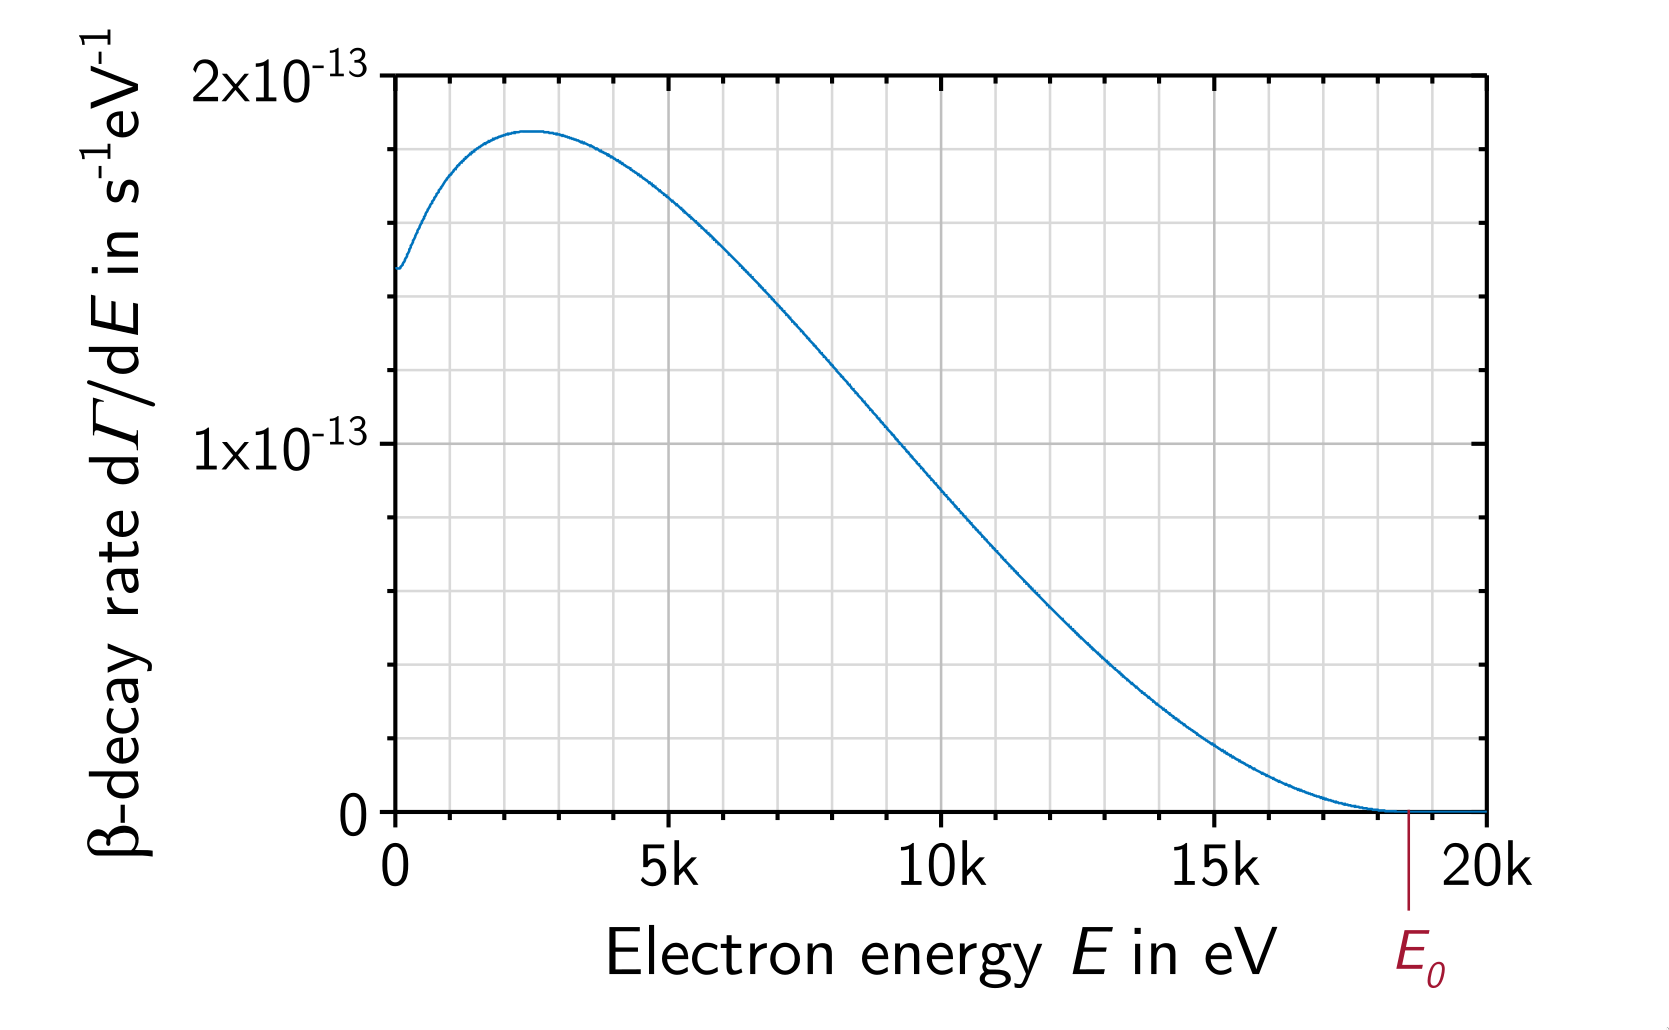
\includegraphics[angle=0,width=\textwidth,clip=0]{beta-spectrum}
	\caption{
		طیف واپاشی بتازای تریتیوم
		$({^{3}_{1}H} \rightarrow {^{3}_{2}He})$
	}
	\label{betaspec}
\end{figure}

این نتیجه خیلی آزار دهنده بود. نیلز بوهر، نه برای اولین بار، آماده بود تا قانون پایستگی انرژی را رها کند. خوشبختانه پاولی دیدگاه عاقلانه‌تری را پیش گرفت و پیشنهاد داد که واپاشی بتازا، دو ذره‌ای نیست و ذره‌ای دیگر باید همراه آن گسیل شود. به دلیل پایستگی بار، این ذره باید خنثی می‌بود و از آنجایی که انرژی الکترون تا مقدار معادله 
(\ref{Emax}) 
بالا می‌رفت، باید بسیار سبک می‌بود. این ایده در ابتدا با شک بسیاری دیده می‌شد تا در سال ۱۹۳۳، انریکو فرمی نظریه‌اش در زمینه واپاشی‌های هسته‌ای را ارائه کرد که ذره پاولی را نیز شامل می‌شد و به این ترتیب، نوترینو متولد شد. امروزه واپاشی بتازا را به صورت زیر می‌نویسیم:
\begin{equation}
n \rightarrow p^{+} + e^{-} + \bar{\nu_{e}}\,.
\end{equation}

در این واکنش می‌بینیم نوترون در اثر واپاشی، به یک پروتون، یک الکترون، و یک پادنوترینوی الکترون تبدیل شده. از آزمایش‌های واپاشی متعدد مشخص می‌شود که ما در واقع بیش از یک نوع نوترینو داریم و نوترینوی پاولی، در واقع شش ذره مختلف بود: نوترینوهای الکترون، موئون و تاو و پاد نوترینوهای متناظرشان.

موئون و تاو ذراتی همانند الکترون هستند با جرم بسیار بیشتر که اندکی پس از ایجاد، به ذرات سبک‌تر وامی‌پاشند. در دهه‌های ۱۹۵۰ و ۱۹۶۰ مشخص  شد که هر کدام از این سه ذره، نوترینوی متناظر خودشان را دارند که فقط در واپاشی‌های متناظر با همان ذره حضور دارند (شکل 
\ref{leptons}).
\begin{figure}
	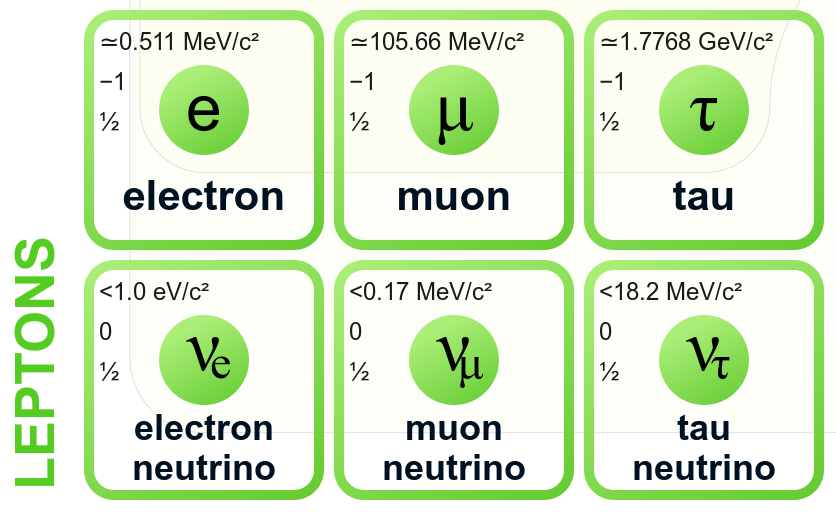
\includegraphics[angle=0,width=0.8\textwidth,clip=0]{leptons}
	\caption{
		خانواده لپتون‌ها. بالا سمت چپ هر ذره، به ترتیب جرم، بار و اسپین آن آمده. هر کدام از این ذرات، پادذره متناسب با خود را نیز دارند.
	}
	\label{leptons}
\end{figure}

قبلا اشاره شد که نوترینوها باید بسیار کم جرم باشند و تا سال‌های بسیار تصور می‌شد بدون جرم هستند چون این فرض محاسبات را بسیار ساده می‌کند. اما امروزه می‌دانیم نوترینوها جرم دارند و هدف این گزارش پرداختن به یکی از مهمترین آزمایش‌های در حال انجامیست که قصد محاسبه این جرم را دارند. در بخش بعدی به پدیده نوسان تونرینو می‌پردازیم که وجود آن، جرم دار بودن نوترینوها را ایجاب می‌کند.


%%===============================SECTION-1===============================%%

%%===============================SECTION-2===============================%%

\section{
نوسانات نوترینو
}
\subsection{
مسئله نوترینوی خورشیدی
}
در نیمه قرن نوزدهم، لرد ریلی محاسبه سن خورشید را به عهده گرفت. او فرض کرد که چشمه انرژی خورشیدی گرانش است و حاصل انرژی جمع شده در اثر فروافتادن مواد از بی نهایت در طول زمان به صورت تابش آزاد می‌شود. ریلی بر اساس آهنگ تابش خورشیدی، بیشینه سن خورشید را بسیار کمتر از سن زمین که زمین شناسان برآورد کرده بودند تخمین زد.

مشکل سن خورشید باقی بود تا در سال ۱۸۹۶، پدیده رادیواکتیویته کشف شد و بکرل و کوری دریافتند که مواد رادیواکتیو مقدار بسیار زیادی گرما گسیل می‌کنند. می‌توان حدس زد که شاید منشا گرمای خورشید مواد رادیواکتیو باشند. اما مشکل این بود که خورشید به طور کامل از هیدروژن و هلیم ساخته شده است و بجز مقدار خیلی خیلی کمی، ماده‌ای رادیواکتیو در طیف آن دیده نشده.

سال ۱۹۲۰ ادینگتون با بررسی اوزان اتمی متوجه شد که جرم چهار اتم هیدروژن اندکی بیشتر از یک اتم هلیوم-۴ است. یعنی با همجوشی چهار اتم هیدروژن و تولید یک اتم هلیوم، به دلیل هم ارزی جرم و انرژی ($E = mc^{2}$)، می‌توان انرژی آزاد کرد. این ساز و کاری بود که ادینگتون برای منشأ انرژی خورشید پیشنهاد کرد. البته او ساز و کار دقیق این همجوشی را نمی‌دانست و باید برای پی بردن به آن تا زمان کشف نوترون و نوترینو صبر می‌کردیم.

در سال ۱۹۳۸ هانس بته مسئله همجوشی را حل کرد و نشان داد دو زنجیره همجوشی می‌تواند وجود داشته باشد. یکی زنجیره CNO (کربن - نیتروژن - اکسیژن) که در ستاره‌های سنگین غالب است و روند همجوشی را تسریع می‌کند. و دیگری زنجیره معروف $pp$ که در (شکل
\ref{pp}) 
نشان داده شده و زنجیره غالب در ستارگان کم جرم و با جرم متوسط همچون خورشید است.


\begin{figure}
	\begin{subfigure}[b]{.33\linewidth}
		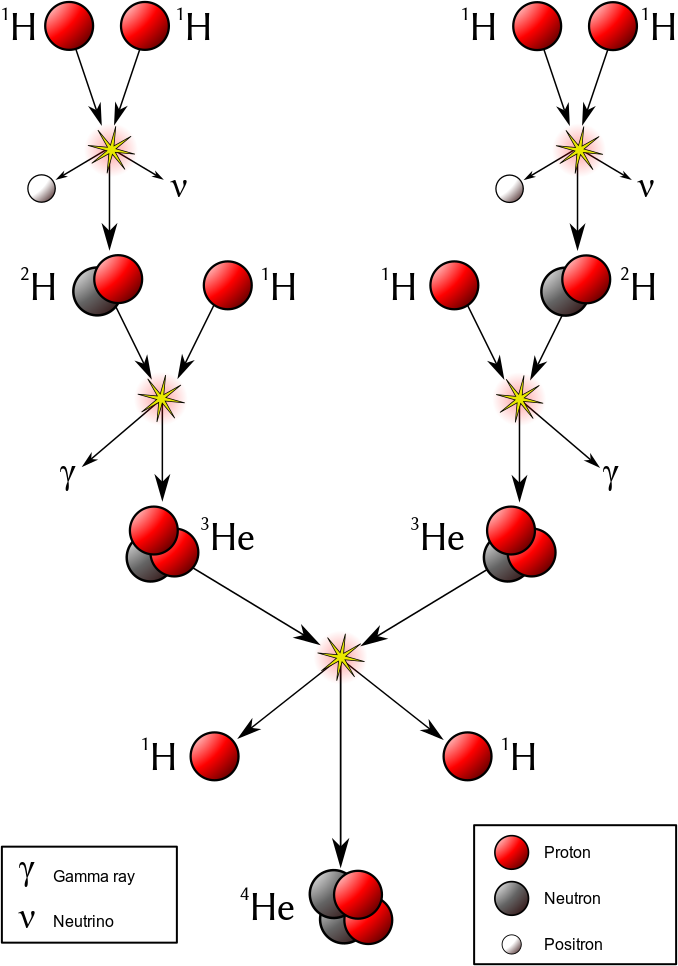
\includegraphics[width=\linewidth]{pp1}
		\caption{
	زنجیره اصلی $pp$	
	}
	\end{subfigure}%
	\begin{subfigure}[b]{.33\linewidth}
		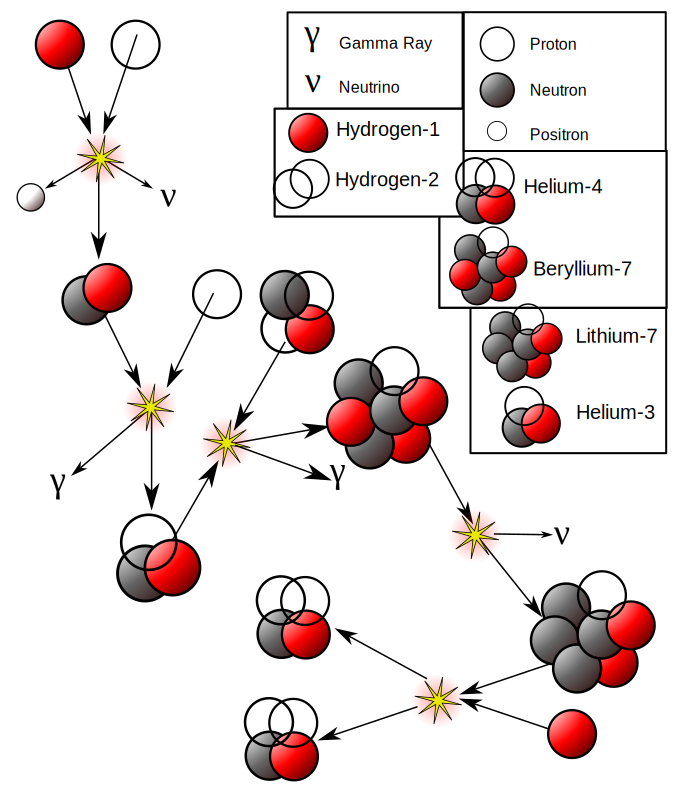
\includegraphics[width=\linewidth]{pp2}
		\caption{
	زنجیره دوم $pp$	
	}
	\end{subfigure}
	\begin{subfigure}[b]{.33\linewidth}
		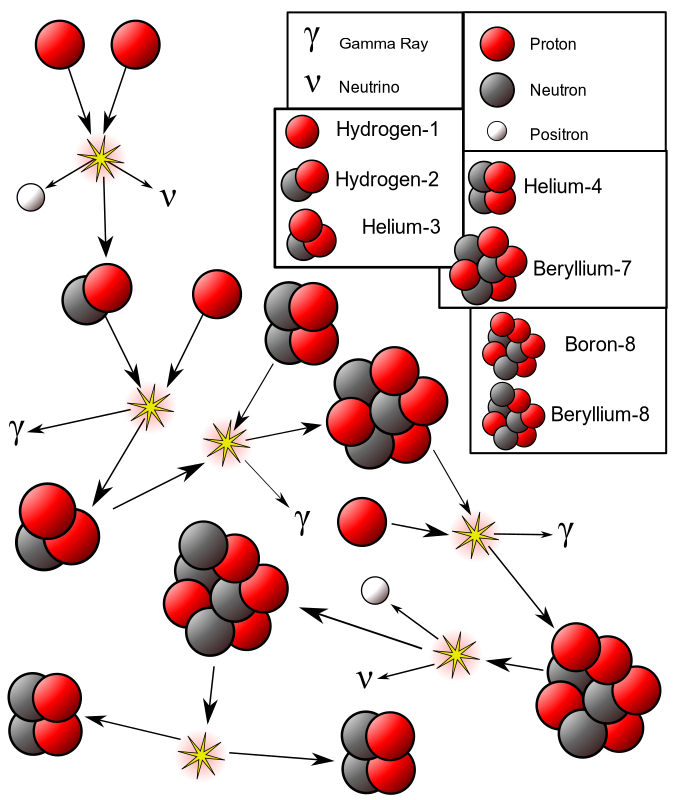
\includegraphics[width=\linewidth]{pp3}
		\caption{
	زنجیره سوم $pp$	
	}
	\end{subfigure}

	\caption{
سه زنجیره پروتون-پروتون	که منبع اصلی انرژی خورشید هستند.
}
	\label{pp}
\end{figure}

جزئیات این زنجیره برای مبحث ما خیلی مهم نیستند. فقط این نکته اهمیت دارد که همه آنها نوترینو آزاد می‌کنند و به دلیل تعداد بالای واکنش‌های همجوشی در خورشید، انتظار تعداد زیادی نوترینو داریم. جان باکال، که بیشترین محاسبات فراوانی نوترینوی خورشیدی را انجام داده می‌گوید در هر ثانیه حدود ۱۰۰ میلیارد نوترینو از هر سانتی‌متر مربع بدن ما می‌گذرد و هنوز آنقدر لطیف اند که می‌توانیم انتظار داشته باشیم که در طول عمرمان یک یا دو برهمکنش نوترینویی در بدن‌مان رخ دهد.

در سال ۱۹۶۸، ری دیویس و همکارانش اولین آزمایش‌ها برای اندازه گیری نوترینوهای خورشیدی را با استفاده از یک مخزن بزرگ کلراین انجام دادند. این مخزن در معدن متروکه هومساک در داکوتای جنوبی ایالات متحده آمریکا قرار دارد. آزمایش‌های نوترینویی را در اعماق زمین انجام می‌دهند که تابش‌های پس زمینه کیهانی حذف شوند. در آزمایش دیویس، یکی از نوترون‌های موجود در کلراین، با یک نوترینوی خورشیدی واکنش می‌دهد و آن را به آرگون تبدیل می‌کند.
\begin{equation}
	\nu_{e} + {^{37}Cl} \rightarrow {^{38}Ar}\,.
\end{equation}

دیویس، هر چند ماه یک بار، مخزن را خالی می‌کرد و اتم‌های آرگون تولید شده را می‌شمرد و این آزمایش را - که در سال ۲۰۰۲ به خاطرش برنده جایزه نوبل شد - برای سال‌ها ادامه داد. تعداد اتم‌های آرگون تولید شده، حدود یک سوم مقدار پیش‌بینی شده بود ( شکل
\ref{davis}).


\begin{figure}
	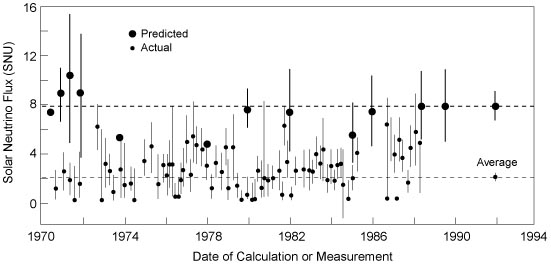
\includegraphics[angle=0,width=0.9\textwidth,clip=0]{davis}
	\caption{
		آزمایش دیویس. دایره‌های بزرگ، شار پیش‌بینی شده نوترینوها را نشان می‌دهند و دایره‌های کوچک، مقادیر اندازه‌گیری شده را.
	}
	\label{davis}
\end{figure}

\subsection{
نوسان‌ها
}
ابتدا در مورد آزمایش دیویس شک‌های زیادی وجود داشت اما آزمایش‌های دیگر نیز آن را تایید کردند. مدل استاندارد خوشیدی نیز با آزمایش‌های دیگر تطبیق خوبی داشت و احتمال غلط بودن آن تا این حد، بسیار کم بود. برونو پونته‌کورو توضیح ساده زیبایی برای مسئله نوترینوی خورشیدی ارائه کرد. او گفت نوترینوهای الکترون که خورشید تولید کرده است، می‌توانند در پرواز به نوترینوهای موئون یا تاو تبدیل شوند که آزمایش دیویس به آنها حساس نبود.

نظریه نوسانات نوترینو، براساس مکانیک کوانتومی حالات آمیخته بنا شده که بسیار به نظریه کلاسیکی نوسانگرهای جفت شده شباهت دارد. محاسبات را برای حالت ساده‌تر دو نوترینو اینجا انجام می‌دهیم و سپس نتایج کلی که برای هر سه نوترینو محاسبه شده را می‌آوریم. حالتی را با دو نوترینوی $\nu_{e}$ و $\nu_{\mu}$ در نظر بگیرید. اگر این دو را بتوان به هم تبدیل کرد، یعنی هیچ کدام ویژه ‌حالت هامیلتونی نیستند و حالت پایای واقعی سیستم، یک ترکیب خطی متعامد از آنهاست.
\begin{equation}\label{nu}
\nu_{1} = cos\theta\,\nu_{\mu} - sin\theta\,\nu_{e}\,,\qquad
\nu_{2} = sin\theta\,\nu_{\mu} + cos\theta\,\nu_{e}\,. 
\end{equation}
بر اساس معادله شرودینگر، این ویژه‌ حالت‌ها وابستگی زمانی به صورت زیر دارند.
\begin{equation}
\nu_{1}(t) = \nu_{1}(0) e^{-iE_{1}t/\hbar}\,,\qquad
\nu_{2}(t) = \nu_{2}(0) e^{-iE_{2}t/\hbar}\,. 
\end{equation}

حال فرض کنید از حالتی که فقط نوترینوی الکترون داریم، شروع کنیم یعنی
\begin{equation}
\nu_{e}(0) = 1\,,\qquad
\nu_{\mu}(0) = 0\,. 
\end{equation}
پس
\begin{equation}
\nu_{1}(0) = -sin\theta\,,\qquad
\nu_{2}(0) = cos\theta\,. 
\end{equation}
و
\begin{equation}
\nu_{1}(t) = -sin\theta e^{-iE_{1}t/\hbar}\,,\qquad
\nu_{2}(t) = cos\theta e^{-iE_{2}t/\hbar}\,. 
\end{equation}
حالا با حل معادله (
\ref{nu}) 
تابع موج 
$\nu_{\mu}$ 
را حساب می‌کنیم.
\begin{equation}
\nu_{\mu}(t) = cos\theta\,\nu_{1}(t) + sin\theta\,\nu_{2}(t) = sin\theta\,cos\theta (-e^{-iE_{1}t/\hbar} + e^{-iE_{2}t/\hbar})\,.
\end{equation}
پس احتمال آنکه نوترینوی الکترون بعد از زمان $t$ به نوترینوی موئون تبدیل شود برابر است با:
\begin{flalign*}
&{|\nu_{\mu}(t)|}^{2} = (sin\theta\,cos\theta)^{2} (-e^{-iE_{1}t/\hbar} + e^{-iE_{2}t/\hbar})(-e^{iE_{1}t/\hbar} + e^{iE_{2}t/\hbar})\\
	&= \frac{sin^{2}(2\theta)}{4}(1 - e^{i(E_{2}-E_{1}t/\hbar)} - e^{-i(E_{2}-E_{1}t/\hbar)} + 1)\\
	&= \frac{sin^{2}(2\theta)}{4} (2 - 2cos\frac{(E_{2}-E_{1})t}{\hbar})\\
	&= \frac{sin^{2}(2\theta)}{4} \times 4 sin^{2}(\frac{E_{2}-E_{1}}{\hbar}t) &&
\end{flalign*}
یا
\begin{equation}
P_{\nu_{e} \rightarrow \nu_{\mu}} = [sin(2\theta)\,sin(\frac{E_{2}-E_{1}}{\hbar}t)]^{2}
\end{equation}

پس مشخص شد که نوترینوی الکترون با گذشت زمان به نوترینوی موئون تبدیل می‌شود و دوباره به صورت سینوسی برمی‌گردد، درست مثل رفت و برگشت بین مدهای عادی در نوسانگرهای جفت شده. در این نظریه، خود نوترینوهای الکترون و موئون، جرم یا انرژی خوش تعریفی ندارند. ویژه حالت‌های $\nu_{1}$ و $\nu_{2}$ به ترتیب جرم‌های $m_{1}$ و $m_{2}$ دارند.
توجه کنید که دو شرط برای رخ دادن نوسانات نوترینو نیاز است: (۱) آنها باید آمیخته باشند و (۲) جرم‌های‌شان یکسان نباشند. پس حداکثر یکی از ویژه جرم‌های نوترینوها می‌تواند صفر باشد.

\subsection{
ماتریس آمیختگی
}
در بخش قبلی، نوسانات دو نوع نوترینو را بررسی کردیم، اما در واقع سه نوع وجود دارد و این ریاضیات را کمی پیچیده‌تر می‌کند. ولی نکته اساسی تغییر نمی‌کند: نوترینوها در نقش ویژه توابع طعم(
$\nu_{e}, \nu_{\mu}, \nu_{\tau}$
) برهمکنش دارند ولی به صورت ویژه حالت‌های هامیلتونی ذره آزاد(
$\nu_{1}, \nu_{2}, \nu_{3}$
) منتشر می‌شوند.

ضرایب آمیختگی را برای سه نوترینو با ماتریس زیر نمایش می‌دهند:
\begin{equation}
\begin{pmatrix}
\nu_{e}    \\
\nu_{\mu}  \\
\nu_{\tau}
\end{pmatrix} = 
\begin{pmatrix}
U_{e1}     & U_{e2}     & U_{e3}     \\
U_{\mu 1}  & U_{\mu 2}  & U_{\mu 3}  \\
U_{\tau 1} & U_{\tau 2} & U_{\tau 3} \\
\end{pmatrix}
\begin{pmatrix}
\nu_{1} \\
\nu_{2} \\
\nu_{3}
\end{pmatrix}
\end{equation}

ظرایب ماتریس $U$ را باید از آزمایشات نوسانات نوترینو به دست آورد. اعداد دقیقی برای ضرایب این ماتریس وجود ندارد اما همانطور که در (شکل 
\ref{flavour})
 نشان داده شده، $\nu_{3}$ ترکیبی تقریبا ۵۰-۵۰ از $\nu_{\mu}$ و $\nu_{\tau}$ است، $\nu_{2}$ تقریبا ترکیبی برابر از سه طعم است و $\nu_{1}$ بیشتر از $\nu_{e}$ تشکیل شده. همچنین می‌دانیم دو تا از ویژه حالت‌های جرم، جرمی نزدیک به هم دارند و یکی از آنها جرمی دور از دو حالت دیگر دارد.
\begin{figure}
	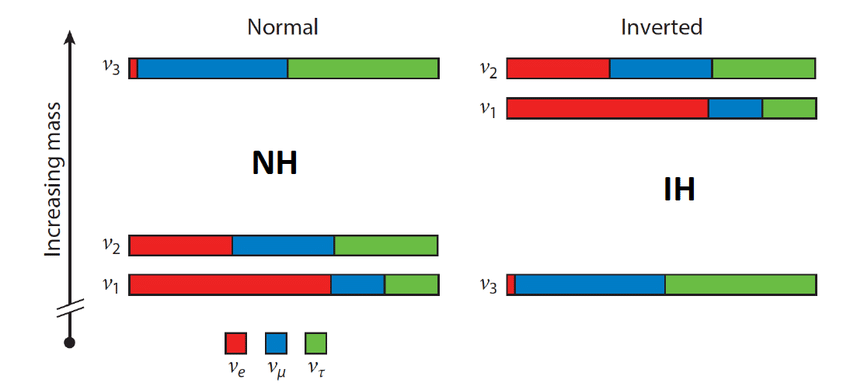
\includegraphics[angle=0,width=\textwidth,clip=0]{neutrino-mass-flavour}
	\caption{
		ترکیب طعمی جرم‌های مختلف نوترینو. دو تا از جرم‌ها به هم خیلی نزدیک هستند و دیگری از آن‌ها دور است. شکل برای هر دو سناریوی ممکن کشیده شده.
	}
	\label{flavour}
\end{figure}


\section{
محاسبه نظری جرم نوترینو
}\label{mass}
در ساده ترین حالت، یعنی واپاشی نوترون (
$n \rightarrow p^{+} + e^{-} + \bar{\nu_{e}}$)
، می‌توان جرم موثر پادنوترینوی الکترون را با یک محاسبه ساده نسبیتی به دست آورد.
\begin{equation}\label{momenun}
P_{n} = P_{p} + P_{\bar{\nu}} + P_{e}\,.
\end{equation}
اینجا 
$P = (\frac{E}{c}, \vec{p})$ 
چاربردار تکانه-انرژی است. $c$ نیز سرعت نور است و انرژی و تکانه به صورت زیر تعریف می‌شوند
\begin{align}\label{energy}
&E = \gamma m c^{2}\\
&\vec{p} = \gamma m \vec{v}
\end{align}
و ماتریس مینکوفسکی $\eta = diag(1, -1, -1, -1)$ است.
می‌توانیم معادله 
\ref{momenun}
 را به صورت زیر تغییر دهیم
\begin{equation}
(P_{n} - P_{e})^{2} = (P_{p} + P_{\bar{\nu}})^{2}
\end{equation}
و با نوشتن چاربردارها در دستگاه سکون نوترون و کمی محاسبه، می‌رسیم به
\begin{equation}
2 m_{n} E_{e} = (m_{n}^{2} + m_{e}^{2} - m_{p}^2 - m_{\bar{\nu}}^{2}) c^{2} - \frac{2 E_{p} E_{\bar{\nu}}}{c^{2}} + 2 \vec{p}_{p} \cdot \vec{p}_{\bar{\nu}}\, .
\end{equation}
با جایگذاری انرژی و تکانه از رابطه 
\ref{energy} 
داریم:
\begin{equation}\label{minimize}
E_{e} = \frac{m_{n}^{2} + m_{e}^{2} - m_{p}^{2} - m_{\bar{\nu}}^{2} - 2 \gamma_{p} \gamma_{\bar{\nu}} m_{p} m_{\bar{\nu}} (1 - \frac{\vec{v}_{p} \cdot \vec{v}_{\bar{\nu}}}{c^{2}})}{2 m_{n}}\,.
\end{equation}

تمام جرم‌ها ثابت هستند پس برای محاسبه $E_{e, max}$ باید جمله آخر رابطه 
\ref{minimize}
 را کمینه کنیم. متغیر $X$ را به صورت زیر تعریف می‌کنیم

\begin{equation}
X = \gamma_{p} \gamma_{\bar{\nu}} (1 - \frac{\vec{v}_{p} \cdot \vec{v}_{\bar{\nu}}}{c^{2}}) = \gamma_{p} \gamma_{\bar{\nu}} (1 - \frac{v_{p} v_{\bar{\nu}} \cos(\theta)}{c^{2}})\,.
\end{equation}
با گرفتن مشتق‌های مرتبه اول و دوم $X$ نسبت به $\theta$، می‌بینیم که
 $\theta = 0$ 
یک کمینه است. پس 
\begin{equation}
X = \gamma_{p} \gamma_{\bar{\nu}} (1 - \frac{v_{p} v_{\bar{\nu}}}{c^{2}}) = \frac{c^{2} - v_{p} v_{\bar{\nu}}}{\sqrt{(c^{2} - v_{p}^{2}) (c^{2} - v_{\bar{\nu}}^{2}})}\,,
\end{equation}
و

\begin{equation}
X^{2} = \frac{c^{4} + v_{p}^{2} v_{\bar{\nu}}^{2} - 2 v_{p} v_{\bar{\nu}} c^{2}}{c^{4} + v_{p}^{2} v_{\bar{\nu}}^{2} - (v_{p}^{2} + v_{\bar{\nu}}^{2}) c^{2}} = \frac{a - 2 x y}{a - (x^{2} + y^{2})} \geq 1 \, .
\end{equation}

حالا اثبات شده که مقدار کمینه متغیر $X$ برابر با $1$ است و

\begin{equation}
E_{e, max} = \frac{m_{n}^{2} + m_{e}^{2} - (m_{p} + m_{\bar{\nu}})^{2}}{2 m_{n}} \, .
\end{equation}

پس جرم موثر نوترینو به صورت زیر محاسبه می‌شود
\begin{equation}
m_{\bar{\nu}} = \sqrt{m_{n}^{2} + m_{e}^{2} - 2 m_{n} E_{e, max}} - m_{p} \, .
\end{equation}

اگر تمام مقادیر بالا با دقت بسیار خوبی مشخص شوند، می‌توانیم با جایگذاری در معادله، جرم نوترینو را به طور مستقیم حساب کنیم. اما چون این مقادیر را نداریم باید طیف کامل انرژی الکترون را در نزدیکی نقطه نهایی به دست بیاوریم. هدف آزمایش KATRIN نیز همین است. در بخش‌های بعدی به توضیح آزمایش KATRIN و خطاهایی که استفاده از معادله ساده بالا را ناممکن می‌کنند می‌پردازیم.



\section{
شرح آزمایش
}
هدف آزمایش KATRIN محاسبه جرم موثر نوترینوی الکترون، با دقتی در حد $0.2~eV$ یعنی یک مرتبه مقداری بهتر از آزمایش‌های قبلی است. برای این کار، باید طیف سنجی دقیقی از طیف الکترون واپاشی بتازای تریتیوم انجام شود. تریتیوم به دلیل در دسترس بودن، نیمه عمر مناسب ($12.5$ سال) و انرژی مناسب نقطه نهایی ($18.6~keV$)، بهترین کاندیدا برای این نوع آزمایش‌هاست. البته آزمایش‌هایی با رنیوم نیز در دنیا در حال انجام هستند.


\begin{figure}
	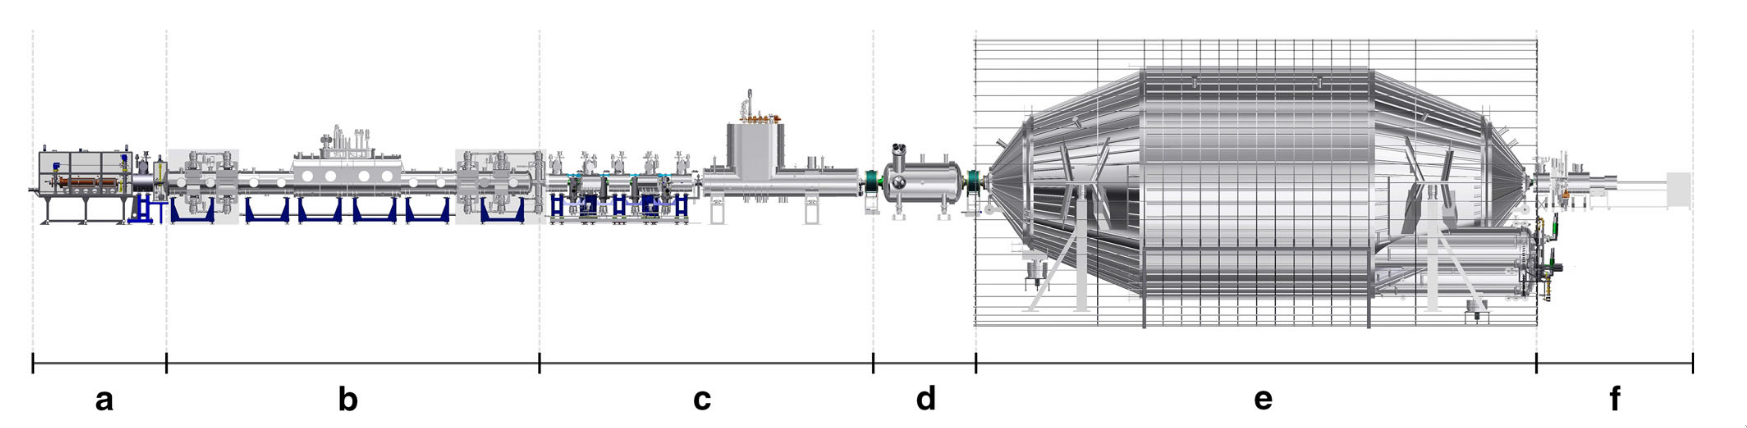
\includegraphics[angle=0,width=\textwidth,clip=0]{setup}
	\caption{
		شمای کلی آزمایشگاه با طول ۷۰ متر. (a) قسمت عقبی برای پایش و کنترل گاز. (b) منبعی که گاز دائما در آن جریان دارد. خلوص و دمای آن روی ۹۵٪ و ۳۰ کلوین ثابت نگه داشته می‌شود. (c) جدا کردن الکترون‌های بتا از گاز و هدایت آنها به سمت آشکار ساز. (d) فیلتر اولیه، الکترون‌های کم انرژی را عبور نمی‌دهد. (e) فیلترهای اصلی در این بخش قرار دارند. با کم و زیاد کردن ولتاژ، طیف بتا را کاوش می‌کند. (f) آشکارسازی که الکترون‌های دریافت شده را می‌شمارد.
	}
	\label{set}
\end{figure}

چیدمان آزمایشگاهی کاترین، یک منبع تریتیوم مولکولی با شدت بالا را به یک طیف‌سنج الکتروستاتیکی از نوع MAC-E متصل می‌کند. این ترکیب همزمان زاویه فضایی بالایی هنگام ورود و باریکه متمرکزی را هنگام خروج الکترون‌ها باعث می‌شود. در شکل
\ref{set} 
 چند زیرسامانه را در دستگاه آزمایش می‌توانید مشاهده کنید که هر کدام کاربرد مخصوصی دارند. در بخش عقبی (a) ترکیب مولکولی مخزن، دما و چگالی بخش‌های مختلف همواره مانیتور می‌شود و مجموعه‌ای از ابزارهای کالیبراسیون برای تنظیم این موارد وجود دارد.
 
منبع تریتیوم بخش (b) حاوی یک باریکه از مولکول‌های 
$T_{2}$ 
با طول $10~m$ و قطر $90~mm$ است و در یک میدان مغناطیسی با شدت $3.6~T$ قرار دارد. مرتباً مولکول‌های حاضر در باریکه، از بخش انتهایی آن خارج شده، خالص سازی می‌شوند و دوباره به چرخه بازمی‌گردند. برای جلوگیری از ورود گاز به بخش طیف سنجی، بخش انتقال (c) طراحی شده است تا شدت گاز را به اندازه ۱۴ مرتبه بزرگی کاهش دهد. فقط الکترون‌های بتا از این بخش عبور می‌کنند و با کمک میدان‌های مغناطیسی به بخش بعدی وارد می‌شوند.
		
در بخش (d) که پیش‌طیف‌نگار (pre-spectrometer) نام دارد، الکترون‌های کم انرژی فیلتر می‌شوند تا الکترون‌های که در نزدیکی نقطه نهایی طیف بتا قرار دارند، به طیف‌نگار اصلی (بخش 
(e
بروند که تحت خلا بسیار شدید و ولتاژ حدود $-18.6~kV$ کار می‌کند. هر دو طیف نگار به صورت فیلترهای MAC-E طراحی شده‌اند و طیف‌نگار اصلی در یک محدوده بسیار کوچک $1~eV$ کار می‌کند. الکترون‌هایی که انرژی کافی دارند از هر دو فیلتر عبور کرده و با آشکار ساز بخش (f) برخورد می‌کنند که شامل ۱۴۸ پیکسل است. طیف بتا با ثبت ولتاژ اعمالی در طیف‌نگار اصلی، رسم می‌شود.

\subsection{
اساس کار فیلتر MAC-E
}
الکترون‌های بتایی که در جهات مختلف منتشر شده‌اند، به صورت بی‌دررو از منبع به بیرون هدایت می‌شوند. الکترون‌ها تحت تاثیر میدان‌های مغناطیسی در یک حرکت سیکلوترونی گیر می‌افتند و در راه رسیدن به آشکارساز انتهای آزمایشگاه، شدت میدان مغناطیسی اعمالی تا چند مرتبه بزرگی کاهش می‌یابد. به دلیل پایستگی انرژی در یک میدانی که تغییرات آرامی دارد، تکانه شعاعی آنها به صورت بی‌دررو به تکانه طولی تبدیل می‌شود. با داشتن یک ولتاژ بزرگ منفی در مرکزش و این توانایی که بیشتر تکانه الکترون‌ها را موازی با محور دستگاه آزمایش می‌کند، فیلتر MAC-E به صورت یک فیلتر انرژی بسیار دقیق کار می‌کند. تنها الکترون‌هایی می‌توانند از این فیلتر عبور کنند، که انرژی اولیه‌شان از ولتاژ منفی اعمالی بیشتر باشد و بقیه الکترون‌ها بازتاب می‌شوند.

همیشه تمام تکانه شعاعی الکترون نمی‌تواند به تکانه طولی تبدیل شود و از آنجایی که آشکارساز نهایی، انرژی الکترون‌های فرودی را نمیتواند تعیین کند، یک خطایی وجود دارد. این خطا که به آن رزولوشن فیلتر می‌گویند، متناسب با حداقل میدان اعمالی و حداکثر میدان اعمالی در مسیر است.
\begin{equation}
\Delta E = \frac{B_{min}}{B_{MAX}} \cdot E \frac{\gamma + 1}{2}\,
\end{equation}
در این معادله E انرژی الکترون و $\gamma$ ضریب نسبیت است. خلاصه‌ای از پارامترهای عملیاتی آزمایش کاترین که چندتا از آنها اینجا معرفی شدند را در جدول 
\ref{param}
 می‌توانید مشاهده کنید.

\begin{table}
	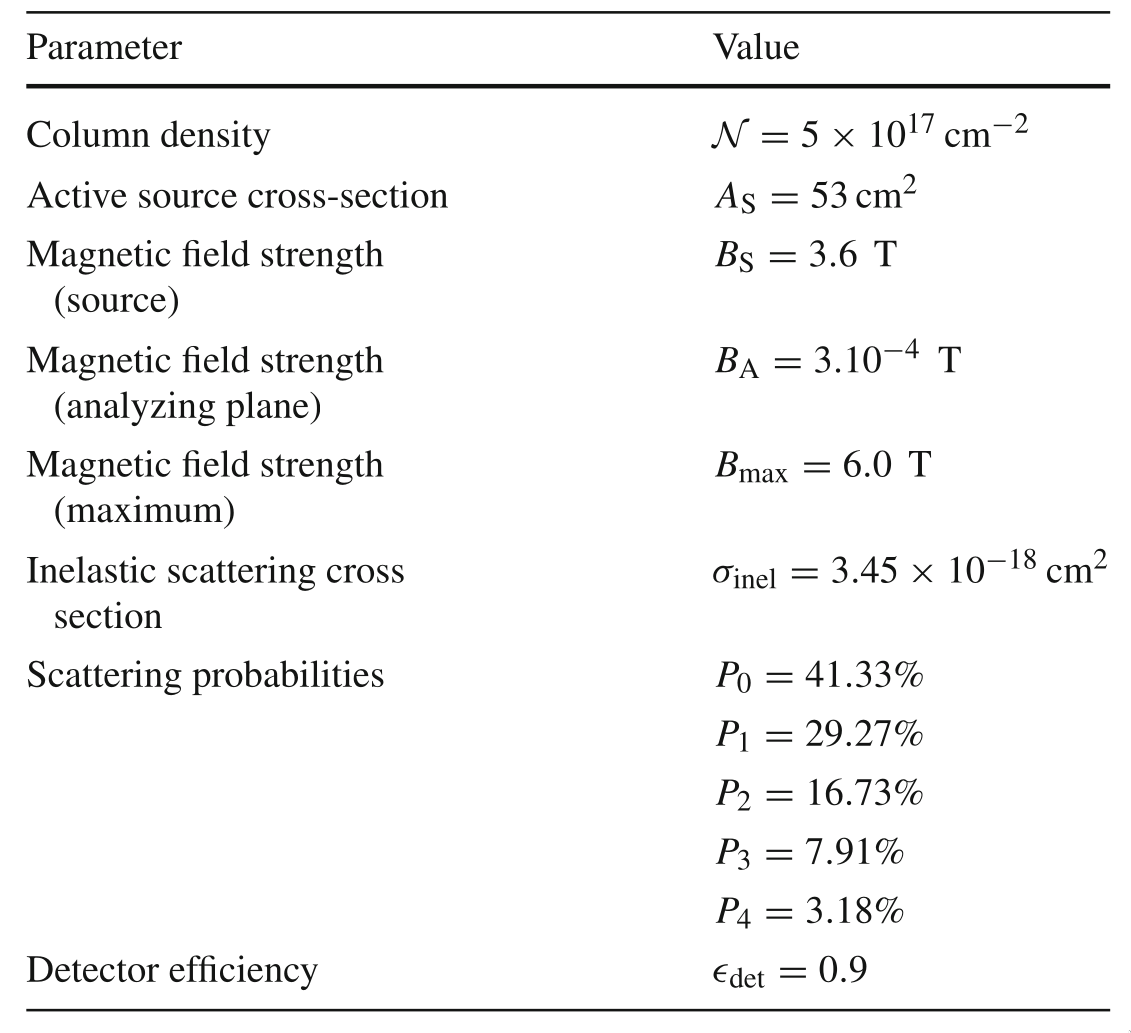
\includegraphics[width=0.7\linewidth]{params}
	\caption{
پارامترهای عملیاتی و محاسبه شده مهم .KATRIN
$B_{A}$ 
همان کمترین مقدار میدان مغناطیسی در طیف‌سنج است.	
}
	\label{param}
\end{table}

\section{
خطاهای آزمایش
}
\begin{table}
	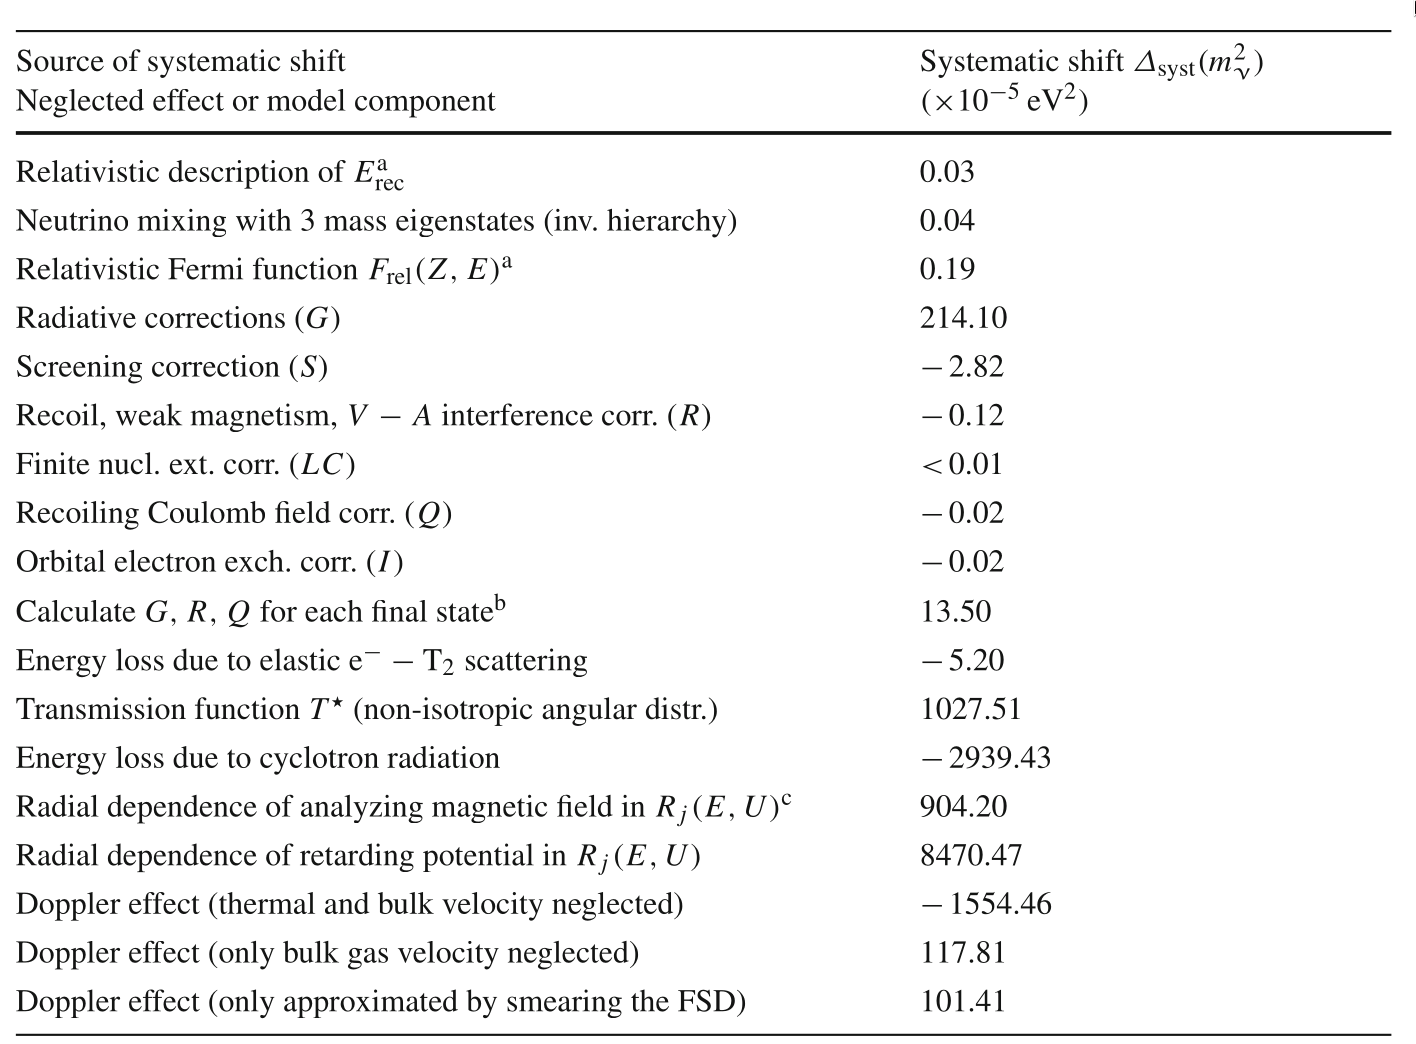
\includegraphics[width=\linewidth]{table1}
	\caption{
		منبع خطاهای سیستماتیک و میزان تاثیرشان روی انرژی نقطه نهایی.	
	}
	\label{error}
\end{table}


در این بخش تعدادی از خطاهای سیستماتیک و آماری آزمایش را بررسی می‌کنیم تا با موانع اندازه گیری جرم نوترینو در شرایط واقعی، بیشتر آشنا شویم. خلاصه‌ای از این خطاها و میزان تاثیرشان روی انرژی نقطه پایانی الکترون، در جدول 
\ref{error} 
آمده.

\subsection{
اثر داپلر
}

یکی از مهمترین اثراتی که باید در نظر گرفته شوند، اثر داپلر است که در اثر حرکت گرمایی گاز تریتیوم در منبع به وجود می‌آید. دمای داخل منبع در ۳۰ کلوین نگه داشته می‌شود که این اثر تاثیر کمتری داشته باشد. اندازه سرعت مولکول‌های گاز در اثر حرکت گرمایی، از یک توزیع ماکسول-بولتزمان پیروی می‌کند. اما اگر فقط سرعت مولکول‌ها در راستای الکترون را در نظر بگیریم، که آن را با برای ایزوتوپی به جرم $M$ با
$v_{M}$ 
نشان می‌دهیم. از یک تابع توزیع گاوسی پیروی می‌کند.
\begin{equation}
g(v_{M}) = \frac{1}{\sqrt{2\pi}\sigma_{v}} \cdot e^{-\frac{1}{2} (\frac{v_{M}}{\sigma_{v}})^{2}}
\end{equation}
در اینجا 
$\sigma_{v} = \sqrt{k_{B}T/M}$.
با انتگرال گرفتن روی تمام زوایای پرتابی که می‌توانند وارد فیلتر شوند، و انجام کمی عملیات جبری، برای توزیع انرژی می‌رسیم به
\begin{equation}
g(E_{cms}, E_{lab}) = \frac{g(v_{M})}{\gamma_{cms} m_{e} v_{e,cms}}\,,
\end{equation}
که اندیس‌های $cms$ و $lab$ به ترتیب نشان دهنده‌ی دستگاه مرکز جرم و آزمایشگاه هستند و داریم
\begin{equation}
v_{M} \approx \frac{v_{e,lab} - v_{e,cms}}{1 - v_{e,lab} \cdot v_{e,cms}/c^{2}}\,.
\end{equation}
پس به این ترتیب خطای استاندارد اثر داپلر به دست می‌آید:
\begin{equation}
\sigma_{E} = \sigma_{v} \gamma_{cms} m_{e} v_{e,cms} = \sqrt{(E_{cms}+2m_{e})E_{cms} \cdot k_{B} T/M}\,.
\end{equation}

برای 
$\sigma_{v} = 203~m/s$ 
و برای مولکول‌های 
$T_{2}$ 
در دمای $T = 30~K$
، و در حالتی که سرعت کل گاز در منبع حدود $13~m/s$ است، اثر داپلر تاثیر بسیار زیادی می‌تواند روی تابع توزیع انرژی داشته باشد. پس حتما باید آن را لحاظ کنیم.

\subsection{
تابش سیکلوترونی
}
الکترون‌ها در مدت زمان عبورشان از منبع تا طیف‌نگار، در اثر حرکت سیکلوترونی انرژی از دست می‌دهند و این افت انرژی در کل طول مسیر برقرار است. برای یک ذره با انرژی جنبشی E که زمان $\Delta t$ در یک میدان مغناطیسی با شدت B حرکت می‌کند، انرژی‌ای که در اثر تابش سیکلوترونی از دست می‌دهد، از رابطه زیر به دست می‌آید:
\begin{equation}
\Delta E^{cycl}_{\bot} = -\frac{q^{4}}{3 \pi c^{3} \epsilon_{0} m_{e}^{3}} \cdot B^{2} . E_{\bot} \frac{\gamma + 1}{2} \cdot \Delta t \,.
\end{equation}
در حالت کلی، تابش سیکلوترونی، مولفه عمودی تکانه را کاهش می‌دهد. در نتیجه برای الکترون‌هایی که با زاویه پرتاب بیشینه وارد طیف‌نگار می‌شوند، بیشینه و برای الکترون‌هایی که موازی با محور آزمایش وارد می‌شوند، صفر است.

برای هندسه پیچیده دخیل در آزمایش کاترین، انرژی تلف شده در اثر تابش سیکلوترونی را با روش‌های مختلف شبیه سازی کردند. این اثر علاوه بر زاویه پرتاب، به مکان شروع الکترون یا همان مکان واپاشی تریتیوم در منبع نیز وابسته است. طبق شبیه سازی‌ها حداکثر انرژی که از این طریق می‌تواند تلف شود، $85~meV$ برای زاویه پرتاب
 $\theta_{MAX} = 50.8^{\circ}$ 
است. این اثر را به عنوان یک شیفت در انرژی نقطه پایانی در نظر می‌گیرند.

\subsection{
اثرات دیگر
}
اثرات دیگری نیز وجود دارند همچون وابستگی شعاعی میدان‌های الکترومغناطیسی دخیل در سیستم و اثرات حضور ایزوتوپ‌های مختلف(
$DT,~D_{2},~HT,~HD,~H_{2},~HeT,~HeD,~HeH$)
که تاثیرات قابل مشاهده‌ای می‌گذارند و باید با محاسبه دقیق و شبیه سازی، میزان اثر آنها و نحوه توزیعشان را حساب کرد.

همچنین اثراتی مانند تابع فرمی نسبیتی و اثر سطح مقطع محدود هسته نیز وجود دارند که به علت تاثیر کوچکشان، می‌توان از آنها چشم پوشی کرد تا حجم محاسبات برای تحلیل داده‌ها کاهش بیابد.

\section{
وضعیت فعلی آزمایش و نگاهی به آینده
}
طراحی آزمایش کاترین در سال ۲۰۰۱ شروع شد و ساخت بخش‌های اصلی آن در سال ۲۰۱۵ به اتمام رسید. در سال ۲۰۱۶، آزمایشی دو هفته‌ای برای تست منبع تریتیوم و محاسبه خطاهای مختلف آزمایش ، به نام First Tritium اجرا شد. ساخت بخش‌های دیگر تا سال ۲۰۱۹ ادامه یافت و اولین داده گیری، روز ۱۰ آوریل ۲۰۱۹ شروع شد. در سپتامبر همان سال، مقاله‌ای منتشر شد که نشان می‌داد حد بالایی برای جرم نوترینو در $1.1~eV$ تعیین شده که پیشرفت قابل توجهی نسبت به $2~eV$ قبلی بود.

\begin{figure}
	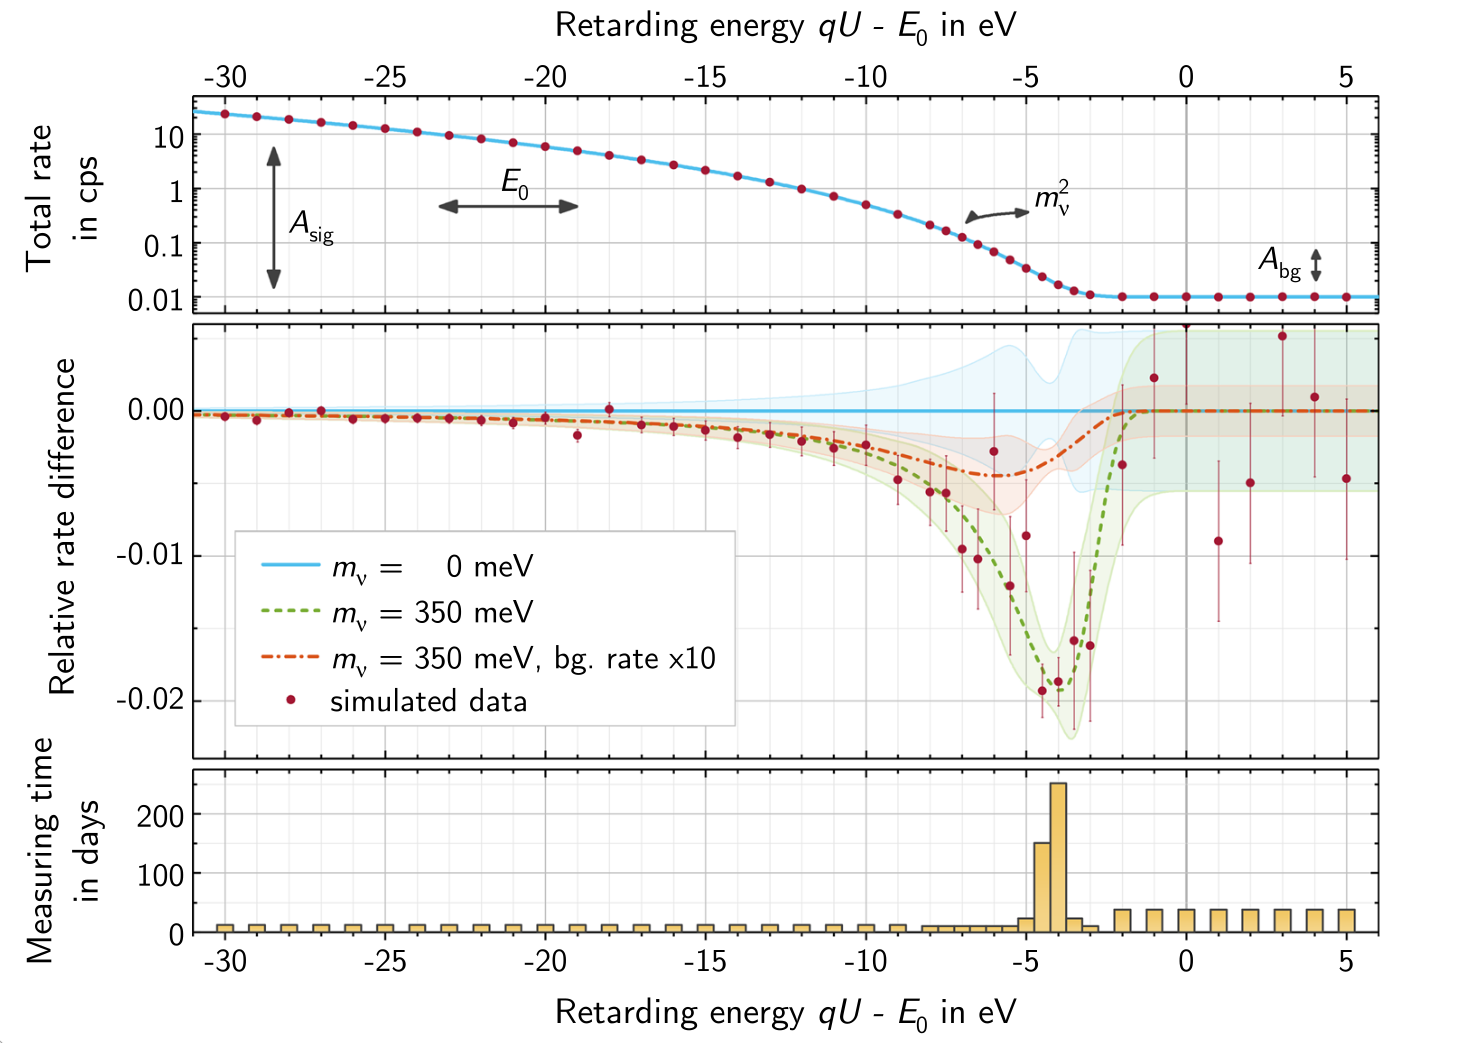
\includegraphics[width=\linewidth]{sim}
	\caption{
		داده‌های شبیه سازی شده برای سه حالت مختلف نوترینوی بی‌جرم، نوترینوی جرم‌دار، نوترینوی جرم دار در صورت وجود تابش زمینه بیش از حد انتظار. همچنین میزان شدت دریافتی کل در آشکارساز و زمان داده گیری در هر پنجره انرژی نشان داده شده.	
}
	\label{sim}
\end{figure}

تیم کاترین امیدوار است تا سپتامبر سال ۲۰۲۰ بتوانند سه داده گیری ۶۵ روزه را به سرانجام برسانند. در نهایت قرار است تا ۱۰۰۰ روز داده گیری در طول ۵ الی ۶ سال انجام شود تا بتوان یا جرم نوترینو را تعیین کرد یا حد بالایی در $0.2~eV$ برای آن گذاشت.

در نمودار
\ref{sim} 
می‌توانید یک نمونه از داده‌های شبیه سازی شده قابل انتظار را ببینید. تصویر بالایی، شدت کل مورد انتظار سیگنال دریافتی در آشکار ساز را برای انرژی‌های کاهنده مختلف نشان می‌دهد. تصویر وسط، تفاوت‌ نمودارهای مورد انتظار برای سه مورد نوترینوی بی‌جرم (خط آبی)، نوترینو با جرم $350~meV$ (نقطه‌چین سبز) و نوترینو با جرم $350~meV$ و شدت نویز زمینه ۱۰ برابر (نقطه‌چین قرمز) را نشان می‌دهد. تصویر پایین زمان‌های داده گیری در هر پنجره انرژی است.

\section{
سخن پایانی
}
من در درس ذرات بنیادی که ترم پیش داشتم، به مبحث نوترینوها علاقه‌مند شدم. البته در سطح مقدماتی این درس که برای دوره کارشناسی می‌گذرانیم، چیز زیادی راجع به نوترینوها نمی‌خوانیم. همین امر باعث شد که پروژه درس مکانیک کوانتومی را فرصتی ببینم برای تحقیق و مطالعه بیشتر در این زمینه تا درک نظری بهتری از ذرات بنیادی به دست آورم.

ابتدا محاسبه‌ای که در بخش 
\ref{mass}
 آمده را انجام دادم و آن را نشان استاد درس ذرات بنیادی‌ام دادم و به پیشنهاد ایشان برای یکی از اعضای تیم کاترین فرستادم. به من گفتند که در آزمایشگاه شرایط خیلی پیچده‌تر است و نیاز به تئوری‌های کامل‌تری با در نظر گرفتن همه جانبه خطاها داریم و تشویقم کردند تا در مورد این آزمایش بیشتر بخوانم.
 
مطالعه در این زمینه، علاوه بر بحث نظری، همانند اینکه چگونه می‌توان از مدل‌های فیزیکی ساده که در کلاس یاد می‌گیریم، به مدل‌های واقعی تر رسید، مرا به چالش‌های آزمایشگاهی و عملی کار نیز علاقه‌مند کرد. در کل انجام این پروژه چیزهای مفیدی به من آموخت و سعی کردم آن بخش‌هایی را که بهتر فهمیده بودم در این گزارش و ارائه نهایی‌ام بیاورم.

بخش‌های مربوط به نوسانات نورترینو عمدتا از کتاب ذرات بنیادی گریفیث
\cite{gr}
 بود. توضیحات مربوط به خود آزمایش از دو مقاله 
\cite{Kleesiek2019} 
و 
\cite{Aker2019} 
گرفته شدند. همچنین از دو مقاله 
\cite{Dragoun2015} 
و 
\cite{Bodine2015}
نیز در نوشتن گزارش استفاده شد.
برای مطالعه بیشتر در زمینه مباحث نظری پشت این مبحث نیز می‌توانید به 
\cite{sim} 
و 
\cite{Agostini2019}
مراجعه نمایید.

%%===============================SECTIONS===============================%%

%%===============================BIBLIOGRAPHY===============================%%

{\bibliographystyle{iut-fa.bst}
%{\bibliographystyle{ieeetr-fa.bst}
%{\bibliographystyle{plainurl}
%{\bibliographystyle{plain-fa.bst}
% \setLTRbibitems
% \resetlatinfont

\DefaultMathsDigits
\begin{singlespace}
%\nocite{*}
\bibliography{library}
\end{singlespace}
%\nocite{*}
%\bibliographystyle{amsplain}
%\bibliography{library}
%\end{document}

%%===============================BIBLIOGRAPHY===============================%%

\end{document}
